\documentclass{article}

\usepackage[a4paper,top=4cm,bottom=3cm,left=2.5cm,right=2.5cm]{geometry}
\usepackage[T1]{fontenc}
\usepackage{lineno}
\usepackage{amsmath}
\usepackage{amssymb}
\usepackage{dsfont} %mathds font
\usepackage{amsfonts}
\usepackage{nicefrac}
\usepackage[dvipsnames]{xcolor}
\usepackage{braket}
\usepackage{physics}
\usepackage{tensor}
\usepackage{enumitem}
\usepackage{mathtools}
\usepackage{hyperref}
\usepackage{cleveref}
\usepackage{imakeidx}
\usepackage{tikz}
\makeindex[columns=2, title=Alphabetical Index, intoc]
\usepackage{enumitem}
\usepackage{cancel}
\usepackage{slashed}
\usepackage{bbold}

\usepackage{tocloft} % Per creare un indice personalizzato

\usepackage[compat=1.1.0]{tikz-feynman}
\usepackage{simpler-wick}

\newcommand{\plogo}{\fbox{$\mathcal{BLT}$}} % Generic dummy publisher logo

%%%%%%%%%%%%%%%%%%%%%%%%%%%%%%%%%%%%% DEFINE BOXES %%%%%%%%%%%%%%%%%%%%%%%%%%%%%%%%%%%%%%%

\tikzstyle{mybox} = [draw=black, very thick, rectangle, rounded corners, inner ysep=5pt, inner xsep=5pt]

\usepackage{mdframed}            % This is the packege to define the style of "Exercise" 
\mdfdefinestyle{theoremstyle}{
	linecolor=black,
	linewidth=1pt, 
	frametitlerule=true, 
	frametitlebackgroundcolor=gray!20, 
	innertopmargin=\topskip,
}
\mdtheorem[style=theoremstyle]{ex}{Exercise}

\newlistof{mdf}{mdf}{Table of Contents} % Per fare in modo che gli ambienti creati con \mdfdefinestyle siano inclusi nell'indice

%%%%%%%%%%%%%%%%%%%%%%%%%%%%%%%%%%% DEFINE SOLUTIONS %%%%%%%%%%%%%%%%%%%%%%%%%%%%%%%%%%%%%

\newenvironment{sol}{
    \par \medskip \noindent 
    \textbf{Solution:} \\[5pt]
    }{\newline \rightline{$\square \qquad$} \newpage}

%%%%%%%%%%%%%%%%%%%%%%%%%%%%%%%%%%%%%%%%%%%%%%%%%%%%%%%%%%%%%%%%%%%%%%%%%%%%%%%%%%%%%%%%%%


\input texmacros.tex



\begin{document}

%----------------------------------------------------------------------------------------
%	TITLE PAGE
%----------------------------------------------------------------------------------------

\begin{titlepage} % Suppresses headers and footers on the title page

	\centering % Centre everything on the title page
	
	\scshape % Use small caps for all text on the title page
	
	\vspace*{\baselineskip} % White space at the top of the page
	
	%------------------------------------------------
	%	Title
	%------------------------------------------------
	
	\rule{\textwidth}{1.6pt}\vspace*{-\baselineskip}\vspace*{2pt} % Thick horizontal rule
	\rule{\textwidth}{0.4pt} % Thin horizontal rule
	
	\vspace{0.75\baselineskip} % Whitespace above the title
	
	{\LARGE EXERCISES\\ OF \\ QUANTUM FIELD THEORY \\} % Title
	
	\vspace{0.75\baselineskip} % Whitespace below the title
	
	\rule{\textwidth}{0.4pt}\vspace*{-\baselineskip}\vspace{3.2pt} % Thin horizontal rule
	\rule{\textwidth}{1.6pt} % Thick horizontal rule
	
	\vspace{2\baselineskip} % Whitespace after the title block
	
	%------------------------------------------------
	%	Subtitle
	%------------------------------------------------
	
	In preparation of the course \emph{Theoretical Physics 1} % Subtitle or further description
    
	
	\vspace*{3\baselineskip} % Whitespace under the subtitle
	
	%------------------------------------------------
	%	Editor(s)
	%------------------------------------------------
	
	Written By
	
	\vspace{0.5\baselineskip} % Whitespace before the editors
	
	{\scshape\Large Andrea  \\ Barontini} % Editor list

    \vspace{0.5\baselineskip} % Whitespace before the editors
	
	{\scshape\Large Niccolò \\ Laurenti} % Editor list

    \vspace{0.5\baselineskip} % Whitespace before the editors
	
	{\scshape\Large Davide Maria \\ Tagliabue} % Editor list
	
	\vspace{5\baselineskip} % Whitespace below the editor list
	
	\textit{Università degli Studi \\ Milano} % Editor affiliation
	
	\vfill % Whitespace between editor names and publisher logo
	
	%------------------------------------------------
	%	Publisher
	%------------------------------------------------
	
	\plogo % Publisher logo
	
	\vspace{0.3\baselineskip} % Whitespace under the publisher logo
	
	%2023 % Publication year
	
	%{\large publisher} % Publisher
    {\large 2023}
    

\end{titlepage}

%----------------------------------------------------------------------------------------

\clearpage
\begin{center}
    \thispagestyle{empty}
    \vspace*{\fill}
    \begin{em}
        <<Polish-born, French-educated Madame Curie, co-discover of radioactivity, she was a hero of science until her hair fell out, her vomit and stool became filled with blood, and she was poisoned to death by her own discovery. With a little hard work, I see no reason why that can't also happen to any of you.>>
    \end{em}
    \vspace{0.5cm} \\
    \hspace{11cm}  - Sheldon Lee Cooper 
    \vspace*{\fill}
\end{center}
\clearpage

%----------------------------------------------------------------------------------------

\listofmdf

\newpage


\begin{ex} \label{Ex1} \addcontentsline{mdf}{mdf}{Exercise \ref{Ex1}}
    Consider a system of $N$ coupled harmonic oscillators with potential
    \begin{equation}
        V = \sum_{i=1}^{N} \frac{\kappa}{2} (q_{i+1} - q_i)^2 \; .
        \label{Eq_ex1_V_def}
    \end{equation}
    Determine the normal coordinates and the eigenvectors of the potential, with boundary conditions $q_0(t) = q_{N+1}(t) = 0$. Determine directly the equations of motion and the normal coordinates in the continuum limit without using the Lagrangian, by taking the continuum limit of the result obtained in the discrete case.
\end{ex}

%%%%%%%%%%%%%%%%%%%%%%%%%%%%%%%%%%%%%%%%%%%%%%%%%%%%%%%%%%%%%%%%%%%%%%%%%%%%%%%%%%%%%%%%%%

\begin{sol}
    The first request of Exercise \ref{Ex1} is to find the normal coordinates and the eigenvectors of the potential of Eq.~\eqref{Eq_ex1_V_def}. Since the solution is rather cumbersome, we refer the reader to Sec.~2.3 of the textbook by David Morin at the link \url{https://scholar.harvard.edu/david-morin/waves}, where an exhaustive discussion on this topic was dedicated.

    Let's see how to solve the second part of the exercise. Since the kinetic energy of a system of $N$ coupled harmonic oscillators corresponds to 
    \begin{equation}
        T =\sum_{i=1}^{N} \frac{m}{2} \dot{q}_i^2 \, ,
    \end{equation}
    the Lagrangian reads
    \begin{equation}
        L = \sum_{i=1}^{N} \left[\frac{m}{2} \dot{q}_i^2 - \frac{\kappa}{2} (q_{i+1}^2 - q_i^2)\right] \, . 
    \end{equation}
    We use it to compute the Euler–Lagrange equation
    \begin{equation}
        \frac{d}{dt} \frac{\partial L}{\partial \dot{q}_k} - \frac{\partial L}{\partial q_k} = 0 \,,
    \end{equation}
    as
    \begin{equation}
    \begin{split}
        \frac{d}{dt} \frac{\partial L}{\partial \dot{q}_k} 
        = & \sum_{i=1}^{N} \frac{m}{2} \frac{d}{dt} \frac{\partial \dot{q}_i^2}{\partial \dot{q}_k} = m \Ddot{q}_k \, , \\
        %
        - \frac{\partial L}{\partial q_k} = & \sum_{i=1}^{N} \frac{\kappa}{2} \frac{\partial}{\partial q_k} (q_{i+1}^2 - q_i^2) = \sum_{i=1}^{N} \kappa (q_{i+1}^2 - q_i^2) (\delta_{i+1,k} - \delta_{ik}) \\
        %
        = &  \kappa (q_k - q_{k-1}) - \kappa(q_{k+1} - q_k) \, , 
    \end{split}
    \end{equation}
    from which we get straightforwardly the discreet equations of motion
    \begin{equation}
        \Ddot{q}_k = \frac{\kappa}{m} (q_{k+1} - q_k) - \frac{\kappa}{m} (q_k - q_{k-1}) \, .
        \label{Eq:question_one_discrete_eom}
    \end{equation}
    
    In order to move to the \emph{continuum limit}, we start by promoting $q_k$ to be a continuous parameter $q(x)$, where $x$ is the position of the $k^{\rm th}$ node along the real axis. Then we define $\Delta x$ as the elongation of the spring between the point $q_k$ and that $q_{k+1}$, i.e.
    \begin{equation}
    \begin{split}
        q_k \mapsto & \, q(t,x) \, , \\
        %
        q_{k+1} \mapsto & \, q(t, x + \Delta x) \, , \\
        %
        q_{k-1} \mapsto & \, q(t, x - \Delta x) \, ,
    \end{split}
    \end{equation}
    according to which Eq.~\eqref{Eq:question_one_discrete_eom} becomes\footnote{We use the handy notation $\partial_t \equiv \partial/\partial t$ and $\partial_x \equiv \partial/\partial x$.}
    \begin{equation}
        \partial_t^2 q(t,x) = \frac{\kappa}{m} \big[q(t, x+\Delta x) - q(t,x)\big] - \frac{\kappa}{m} \big[q(t,x) - q(t, x-\Delta x)\big] \, .
        \label{Eq_Ex1_qdotdot_def}
    \end{equation}
    Assuming $q(t,x)$ smooth enough to have a well defined second derivative in $x$, we can expand the r.h.s.~of Eq.~\eqref{Eq_Ex1_qdotdot_def} in series of $\Delta x \ll 1$ and get
    \begin{equation}
    \begin{split}
        \partial_t^2 q(t,x)|_{\Delta x \ll 1} = & \; \frac{\kappa}{m} \left[q(t,x) + \Delta x \partial_x q(t,x) + \frac{1}{2}(\Delta x)^2 \partial_x^2 q(t,x) - q(t,x) + \mathcal{O}(\Delta x)^3\right] \\
        %
        & - \frac{\kappa}{m} \left[q(t,x) - q(t,x) - \Delta x \partial_x q(t,x) + \frac{1}{2}(\Delta x)^2 \partial_x^2 q(t,x) - q(t,x) + \mathcal{O}(\Delta x)^3\right] \\
        %
        = & \; \frac{\kappa}{m} (\Delta x)^2 \partial_x^2 q(t,x) + \mathcal{O}(\Delta x)^3 \, .
    \end{split}
    \end{equation}
    Finally, by defining $\omega_c$ as
    \begin{equation}
        \omega_c^2 \define \frac{\kappa \Delta x}{m/ \Delta x} = \frac{\kappa_c}{\delta m}  
        \label{Eq_Ex1_omega_c_def}
    \end{equation}
    we find that Eq.~\eqref{Eq:question_one_discrete_eom} can be rewritten in the continuum limit as
    \begin{equation}
        \big(\partial_t^2 - \omega_c^2 \partial_x^2\big) \, q(t,x) = 0 \, .    
    \end{equation}
    This proves that $q(t,x)$ must satisfy the \emph{wave equation}. 

    It remains only to understand whether $\omega_c$ of Eq.~\eqref{Eq_Ex1_omega_c_def} is well defined when $\Delta x \to 0$. In this regard, we point out that:
    \begin{itemize}
        \item $\delta m = m/\Delta x$ is the \textit{mass density} of the new continuum system, which is clearly finite;
    
        \item if one cuts a spring in half, it doubles its stiffness. If we then cut the spring into many pieces, each of length $\Delta x$, we expect the stiffness to become proportional to $\kappa \propto 1/\Delta x$, which diverges for $\Delta x \to 0$. It follows that $\kappa_c = \kappa \Delta x$ must be finite in this limit. 
    \end{itemize}
    Therefore we conclude stating that $\omega_c$ is finite and and well-defined in the limit $\Delta x \to 0$.
\end{sol}
\begin{ex} \label{Ex2} \addcontentsline{mdf}{mdf}{Exercise \ref{Ex2}}
	Consider the Lagrangian density
	\begin{equation}
		\mathcal{L} = \partial_\mu \phi^* \partial^\mu \phi - m^2 \abs{\phi}^2 \; ,
	\end{equation}
	where $\phi(x)$ is a complex classical field. Derive the classical equations of motion and solve them using the method of normal coordinates.
\end{ex}

%%%%%%%%%%%%%%%%%%%%%%%%%%%%%%%%%%%%%%%%%%%%%%%%%%%%%%%%%%%%%%%%%%%%%%%%%%%%%%%%%%%%%%%%%%

\begin{sol}
	In order to derive the classical equations of motion, we need to apply the Euler-Lagrange equations to both $\phi$ and $\phi^{*}$, i.e.
	\begin{equation}
		\begin{split}
			\partial_{\mu}\frac{\partial \mathcal{L}}{\partial(\partial_{\mu}\phi)} &- \frac{\partial \mathcal{L}}{\partial \phi} =  0 \, ,\\
			%
			\partial_{\mu}\frac{\partial \mathcal{L}}{\partial(\partial_{\mu}\phi^{*})} &- \frac{\partial \mathcal{L}}{\partial \phi^{*}} =  0 \, ,
		\end{split}
	\end{equation}
	which, after computing the derivatives, yield
	\begin{equation}
		\begin{split}
			& \partial_{\mu}\partial^{\mu} \phi^{*} + m^{2}\phi^{*} = (\square + m^{2}) \phi^{*} = 0 \, , \\ 
			%
			& \partial_{\mu}\partial^{\mu} \phi + m^{2}\phi = (\square + m^{2}) \phi = 0 \, .
			\label{eq_ex2_KG_eqs}
		\end{split}
	\end{equation}
	Thus, we find that $\phi$ (and, of course, $\phi^*$ as well) satisfies the so-called \emph{Klein–Gordon equation} (KG). 
	
	Now, let's discuss how we can solve it. 
	We write $\phi(x) = \phi(t,\vx)$ in the Fourier space of $\vx$, i.e.,
	\begin{equation}
		\phi(t,\vx) = \int \frac{\rmd^{3} \vp}{(2\pi)^{3}} \, e^{i \vp \cdot \vx}\phi(t,\vp) \,.
		\label{eq_ex2_eq_fourier_1}
	\end{equation}
	The KG equation becomes (recall that $\partial_\mu \partial^\mu = \partial_t^2 - \vgrad^2$)
	\begin{equation}
		(\partial_{\mu}\partial^{\mu} + m^{2} ) \phi(t,\vx)
		=
		\int \frac{\rmd^{3} \vp}{(2\pi)^{3}} \, e^{i \vp \cdot \vx} (\partial_t^2 + \vp^2 + m^2) \phi(t,\vp)
		=
		0 \,,
	\end{equation}
	which implies
	\begin{equation}
		\partial_t^2 \phi(t,\vp) = - \Ep^2 \, \phi(t,\vp) \,,
		\qquad
		\Ep \define \sqrt{\vp^2 + m^2} \,. 
		\label{eq_ex2_eq_fourier_2}
	\end{equation}
	Notice that $\Ep$ is the relativistic energy of the field $\phi$. 
	The general solution of Eq.~\eqref{eq_ex2_eq_fourier_2} reads 
	\begin{equation}
		\phi(t,\vp) = A(\vp) \, e^{-i \Ep t} + B(\vp) \, e^{i \Ep t} \,, 
		\label{eq_ex2_eq_fourier_3}
	\end{equation}
	where $A(\vp)$ and $B(\vp)$ are two distinct time-independent complex functions.
	Substituting this result into Eq.~\eqref{eq_ex2_eq_fourier_1}, we obtain
	\begin{equation}
		\begin{split}
			\phi(t,\vx) & = \int \frac{\rmd^{3} \vp}{(2\pi)^{3}} \big( A(\vp) \, e^{-i \Ep t + i \vp \cdot \vx} + B(\vp) \, e^{i \Ep t + i \vp \cdot \vx} \big)
			\\
			& = \int \frac{\rmd^{3} \vp}{(2\pi)^{3}} \big( A(\vp) \, e^{-i \Ep t + i \vp \cdot \vx} + B(-\vp) \, e^{i \Ep t - i \vp \cdot \vx} \big) \,,
		\end{split}
	\end{equation}
	where in the second line we replaced the variable of integration as $\vp \mapsto - \vp$. 
	At this point, we redefine the functions $A(\vp)$ and $B(\vp)$ as follows:
	\begin{equation}
		A(\vp) \define \frac{a_{\vp}}{\sqrt{2\Ep}} \,,
		\qquad
		B(-\vp) \define \frac{b_{\vp}^*}{\sqrt{2\Ep}} \,,
	\end{equation}
	where the prefactor $1/\sqrt{2\Ep}$ will turn out to be a very useful choice of normalization in quantizing fields.    
	We point out that there is no specific reason to write $b_{\vp}^*$ instead of $b_{\vp}$ at this stage. 
	However, in the quantization of the fields, we will see that $a_{\vp}$ and $b_{\vp}$ will be promoted to operators acting on Hilbert spaces, specifically $b_{\vp} \mapsto \bdes_{\vp}$ and $b_{\vp}^* \mapsto \bcon_{\vp}$. 
	So, we choose $b_{\vp}^*$ to represent a classical solution in a form ready for quantization.
	Finally, we introduce the four-momentum $p^\mu$ defined as
	\begin{equation}
		p^\mu \define (\Ep, \vp) \,,
	\end{equation}
	such that the time component reads $p^0 = \Ep$. 
	This is equivalent to requiring $p^\mu$ to satisfy the equation $p^2 = (p^{0})^{2} - \vp^2 = m^2$. 
	Therefore, the general solution of the KG equation from Eq.~\eqref{eq_ex2_KG_eqs} corresponds to
	\begin{equation}
		\phi(x) = \int \frac{\rmd^{3} \vp}{(2\pi)^{3} \sqrt{2 \Ep}} \eval{(a_{\vp} \, e^{- ipx} + b_{\vp}^* \, e^{ipx})}_{p^{0} = \Ep} \,.
	\end{equation}
	
	Before concluding, we observe that a complex scalar field $\phi$ possesses two degrees of freedom and can be expressed as a combination of two real scalar fields, $\phi_1$ and $\phi_2$:
	\begin{equation}
		\phi(x) = \frac{\phi_1(x) + i \phi_2(x)}{\sqrt{2}} \,,
		\qquad
		\phi^*(x) = \frac{\phi_1(x) - i \phi_2(x)}{\sqrt{2}} \,.
	\end{equation}
	One can freely rewrite the Lagrangian density $\mathcal{L}(x)$ in terms of $\phi_{1,2}$ as:
	\begin{equation}
		\mathcal{L}(x) = \frac{1}{2} \partial_\mu \phi_1 \partial^\mu \phi_1 + \frac{1}{2} \partial_\mu \phi_2 \partial^\mu \phi_2 - \frac{m^2}{2} \big(\phi_1^2 + \phi_2^2\big) \,,
	\end{equation}
	and then derive the equations of motion for $\phi_{1,2}$. This task is left as an exercise for the reader.
\end{sol}
\begin{ex} \label{ex_3} \addcontentsline{mdf}{mdf}{Exercise \ref{ex_3}}
    (...)
\end{ex}

%%%%%%%%%%%%%%%%%%%%%%%%%%%%%%%%%%%%%%%%%%%%%%%%%%%%%%%%%%%%%%%%%%%%%%%%%%%%%%%%%%%%%%%%%%

\begin{sol}
    (...)
\end{sol}
\begin{ex} \label{ex_4} \addcontentsline{mdf}{mdf}{Exercise \ref{ex_4}}
    Show that requiring invariance of the metric upon Lorentz transformations
    \begin{equation}
        \tensor{\Lambda}{^\mu_\nu} \tensor{\Lambda}{^\rho_\sigma} \g^{\nu \sigma} = \g^{\mu \rho} \, ,
        \label{Eq_Ex4_Lambda_prop_1}
    \end{equation}
    and writing the infinitesimal transformation in terms of its generators $J_{\rho \sigma}$
    \begin{equation}
    \label{lorentz_algebra1}
        \tensor{\Lambda}{^\mu_\nu} = \tensor{\g}{^\mu_\nu} - \frac{i}{2} \omega^{\rho \sigma} \tensor{(J_{\rho \sigma})}{^\mu_\nu} \, ,
    \end{equation}
    completely fixes the explicit form of the generators, viewed as $4 \times 4$ Lorenz matrices $\tensor{(J_{\rho \sigma})}{^\mu_\nu}$, and determine their explicit expression. 
\end{ex}

%%%%%%%%%%%%%%%%%%%%%%%%%%%%%%%%%%%%%%%%%%%%%%%%%%%%%%%%%%%%%%%%%%%%%%%%%%%%%%%%%%%%%%%%%%

\begin{sol}
    Let $\Lambda$ and $\omega$ be an element of the Lorentz group and of the Lorentz algebra respectively. The Eq.~\eqref{lorentz_algebra1} states that
    \begin{equation}
        \tensor{\Lambda}{^\mu_\nu} = \tensor{\g}{^\mu_\nu} + \tensor{\omega}{^\mu_\nu} + \mathcal{O}(\omega^2) \, .
    \end{equation}
    Substituting this identity in Eq.~\eqref{Eq_Ex4_Lambda_prop_1} we obtain
    \begin{equation}
    \begin{split}
        & \big[\tensor{\g}{^\mu_\nu} + \tensor{\omega}{^\mu_\nu} + \mathcal{O}(\omega^2)\big] \big[\tensor{\g}{^\rho_\sigma} + \tensor{\omega}{^\rho_\sigma} + \mathcal{O}(\omega^2)\big] \g^{\nu \sigma} \\
        %
        = & \, \g^{\mu \rho} + \tensor{\omega}{^\mu_\nu} \tensor{\g}{^\rho_\sigma} \g^{\nu \sigma} + \tensor{\omega}{^\rho_\sigma} \tensor{\g}{^\mu_\nu} \g^{\nu \sigma} + \mathcal{O}(\omega^2) \\
        %
        = & \, \g^{\mu \rho} + \omega^{\mu \rho} + \omega^{\rho \mu} + \mathcal{O}(\omega^2) \\
        = & \, \g^{\mu\rho} \, ,
    \end{split}
    \end{equation}
    from which we find
    \begin{equation}
        \omega^{\mu \rho} = - \omega^{\rho \mu} \, .
    \end{equation}
    Therefore, a generic element of the Lorentz algebra in the vector representation ($4 \times 4$ matrices) with both high (or low) indices must be \textit{totally antisymmetric}. This implies that the Lorentz algebra necessarily has 6 generators, i.e.
    \begin{equation}
        \omega_{\mu \nu} = 
        \begin{pmatrix}
            0          & \alpha     & \beta    & \gamma \\
            - \alpha   & 0          & \delta   & \epsilon \\
            -\beta     & - \delta   & 0        & \theta \\
            - \gamma   & - \epsilon & - \theta & 0 
        \end{pmatrix} ,
    \end{equation}
    or, written in a more useful way as far as it concerns, 
    \begin{equation}
        \tensor{\omega}{^\mu_\nu} = \g^{\mu\sigma} \omega_{\sigma \nu} = 
        \begin{pmatrix}
            0        & \alpha   & \beta    & \gamma \\
            \alpha   & 0        & - \delta & - \epsilon \\
            \beta    & \delta   & 0        & -\theta \\
            \gamma   & \epsilon & \theta & 0 
        \end{pmatrix} \, .
    \end{equation}
    Basically $\tensor{\omega}{^\mu_\nu}$ is
    \begin{itemize}
        \item symmetric in $(0i)$ and $(i0)$ indices, i.e.
        \begin{equation}
            \tensor{\omega}{^0_i} = \tensor{\omega}{^i_0} \, ,
        \end{equation}
    
        \item antisymmetric in the spatial entries
        \begin{equation}
            \tensor{\omega}{^i_j} = - \tensor{\omega}{^j_i} \, . 
        \end{equation}
    \end{itemize}
    This completely fixes the Lorentz algebra. One can show that $\tensor{\omega}{^0_i}$ correspond to the Lorentz boosts $K^i$, while the antisymmetric part $\tensor{\omega}{^i_j}$ to rotations $\tensor{J}{^i_j}$. 
    
    Let's now see how generators $J^{\rho\sigma}$ appears in the theory. Since $\omega_{\rho \sigma}$ is antisymmetric, we can derive the following identity
    \begin{equation}
        \tensor{\omega}{^\mu_\nu} = \g^{\mu\rho} \tensor{\delta}{^\sigma_\nu} \omega_{\rho \sigma} = \frac{1}{2} \g^{\mu\rho} \tensor{\delta}{^\sigma_\nu} (\omega_{\rho \sigma} - \omega_{\sigma \rho}) = \frac{1}{2} \omega_{\rho \sigma} (\g^{\mu \rho} \tensor{\delta}{^\sigma_\nu} - \g^{\mu \sigma} \tensor{\delta}{^\rho_\nu}) \, .
    \end{equation}
    We are thus free to introduce an antisymmetric tensor $J^{\rho\sigma}$, defined as
    \begin{equation}
        \tensor{(J^{\rho\sigma})}{^\mu_\nu} \define i (\g^{\mu \rho} \tensor{\delta}{^\sigma_\nu} - \g^{\mu \sigma} \tensor{\delta}{^\rho_\nu}) \, , 
        \label{Eq_Ex4_Jmunu_def}
    \end{equation}
    such that
    \begin{equation}
        \tensor{\omega}{^\mu_\nu} = - \frac{i}{2} \omega_{\rho\sigma}\tensor{(J^{\rho\sigma})}{^\mu_\nu} \, .
    \end{equation}
    The definition of these ``new'' generators $J^{\rho\sigma}$ completely determines the Lorentz algebra.
\end{sol}
\begin{ex} \label{Ex_5} \addcontentsline{mdf}{mdf}{Exercise \ref{Ex_5}}
    Derive the Lorentz algebra, i.e.\ the commutation relations
    \begin{equation}
    \label{lorentz_algebra}
        \left[ J^{\mu \nu}, J^{\rho \sigma}\right] = i\left( \g^{\mu \sigma}J^{\nu \rho} + \g^{\nu \rho} J^{\mu \sigma} - \g^{\mu \rho} J^{\nu \sigma} - \g^{\nu \sigma}J^{\mu \rho} \right)
    \end{equation}
    \begin{enumerate}[label=\alph*)]
        \item using the explicit form of the generators found in Exercise \ref{ex_4}, 
        \item from the relation $D(\Lambda)^{-1} D(\Lambda') D(\Lambda) = D(\Lambda^{-1} \Lambda' \Lambda)$, which holds for any Lorentz representation $D(\Lambda)$ in the case of infinitesimal transformation (see Problem 1.11-b of V.~Radovanovi\'c's book \emph{Problem Book Quantum Field Theory}).
    \end{enumerate}
\end{ex}

%%%%%%%%%%%%%%%%%%%%%%%%%%%%%%%%%%%%%%%%%%%%%%%%%%%%%%%%%%%%%%%%%%%%%%%%%%%%%%%%%%%%%%%%%%

\begin{sol}
    \begin{enumerate}[label=\alph*)]
        \item We proceed inserting the explicit expression of $J^{\mu \nu}$ (see Eq.~\eqref{Eq_Ex4_Jmunu_def} in Problem \ref{ex_4}) inside Eq.~\eqref{lorentz_algebra}. After some algebraic manipulations, we obtain
        \begin{align}
            \tensor{[J^{\mu\nu}, J^{\rho \sigma}]}{^\alpha_\beta} ={}& (\g^{\mu\alpha}\tensor{\delta}{^\nu_\gamma} - \g^{\nu\alpha}\tensor{\delta}{^\mu_\gamma})(\g^{\rho\gamma}\tensor{\delta}{^\sigma_\beta} - \g^{\sigma\gamma}\tensor{\delta}{^\rho_\beta}) - (\g^{\rho\alpha}\tensor{\delta}{^\sigma_\gamma} - \g^{\sigma\alpha}\tensor{\delta}{^\rho_\gamma})(\g^{\mu\gamma}\tensor{\delta}{^\nu_\beta} - \g^{\nu\gamma}\tensor{\delta}{^\mu_\beta}) \notag \\
            %
            ={}& - \Bigl[ g^{\mu \alpha} g^{\rho \nu} \delta^\sigma{}_\beta - g^{\mu \alpha} g^{\sigma \nu} \delta^\rho{}_\beta -g^{\nu \alpha} g^{\rho \mu} \delta^\sigma{}_\beta + g^{\nu \alpha} g^{\sigma \mu} \delta^\rho{}_\beta \notag \\
            %
            & - \g^{\rho \alpha} g^{\mu \sigma} \tensor{\delta}{^\nu_\beta} + \g^{\rho \alpha} \g^{\sigma \nu} \tensor{\delta}{^\mu_\beta} + \g^{\sigma \alpha} \g^{\rho \mu} \tensor{\delta}{^\nu_\beta} - \g^{\sigma \alpha} \g^{\nu \rho} \tensor{\delta}{^\mu_\beta} \Bigr] \notag \\
            %
            ={}& -i \Bigl[ (-i)\g^{\mu \sigma}\bigl(\g^{\nu \alpha} \tensor{\delta}{^\rho_\beta} - \g^{\rho \alpha} \tensor{\delta}{^\nu_\beta} \bigr) + (-i) \g^{\nu \rho}\bigl(\g^{\mu \alpha} \tensor{\delta}{^\sigma_\beta} - \g^{\sigma \alpha} \tensor{\delta}{^\mu_\beta} \bigr) \notag \\
            %
            & - (-i) \g^{\mu \rho}\bigl(\g^{\nu \alpha} \tensor{\delta}{^\sigma_\beta} - \g^{\sigma \alpha} \tensor{\delta}{^\nu_\beta} \bigr) - (-i)\g^{\nu \sigma}\bigl(\g^{\mu \alpha} \tensor{\delta}{^\rho_\beta} - \g^{\rho \alpha} \tensor{\delta}{^\mu_\beta} \bigr)\Bigr] \notag \\
            %
            ={}& i \tensor{\big( \g^{\mu \sigma} J^{\nu \rho} + \g^{\nu \rho} J^{\mu \sigma} - \g^{\mu \rho} J^{\nu \sigma} - \g^{\nu \sigma} J^{\mu \rho} \big)}{^\alpha_\beta} \, ,
        \end{align}
        which proves Eq.~\eqref{lorentz_algebra}. \\

        \item Let $\Lambda'$ be an infinitesimal Lorentz transformations $\Lambda' = \id + \omega'$ ($\omega'$ is a term of the Lorentz algebra) and let $D(\Lambda)$ be the representation of any infinitesimal Lorentz transformation $\Lambda$, i.e.
        \begin{equation}
            D(\Lambda) = \id - \frac{i}{2} \omega_{\mu \nu} J^{\mu \nu} \, .
            \label{Eq_Ex5_DLambda_def}
        \end{equation}
        Consider $\Lambda'' = \Lambda^{-1} \Lambda' \Lambda$. Using the expansion of $\Lambda'$, we find
        \begin{equation}
            \Lambda'' = \Lambda^{-1} \Lambda' \Lambda 
            %
            = \id + \Lambda^{-1} \omega' \Lambda \, .
        \end{equation}
        Notice that $\Lambda^{-1} \omega' \Lambda$ is the infinitesimal expansion of $\Lambda''$, therefore using Eq.~\eqref{Eq_Ex5_DLambda_def} we get
        \begin{equation}
            D(\Lambda'') 
            %
            = \id + \Lambda^{-1} \omega' \Lambda = \id - \frac{i}{2} (\Lambda^{-1} \omega' \Lambda)_{\mu\nu} J^{\mu\nu}
            %
            = \id - \frac{i}{2} J^{\mu\nu} \tensor{(\Lambda^{-1})}{_\mu^\rho} \tensor{\Lambda}{^\sigma_\nu} \omega'_{\rho\sigma} \, .
            \label{Eq_Ex5_D(Lambda'')}
        \end{equation}
        On the other hand, the identity $D(\Lambda'') = D(\Lambda^{-1} \Lambda' \Lambda) = D(\Lambda)^{-1} D(\Lambda') D(\Lambda)$ holds, and the r.h.s.~corresponds to 
        \begin{equation}
            D(\Lambda)^{-1} D(\Lambda') D(\Lambda)
            %
            = D^{-1}(\Lambda) \left(\id - \frac{i}{2} \omega'_{\rho \sigma} J^{\rho \sigma}\right) D(\Lambda)
            %
            \equiv \id - \frac{i}{2} D^{-1}(\Lambda) J^{\rho\sigma} D(\Lambda)  \omega'_{\rho\sigma} \, .
        \end{equation}
        So, comparing the above r.h.s.~with that of Eq.~\eqref{Eq_Ex5_D(Lambda'')}, we find\footnote{Here we use Eq.~\eqref{Eq_Ex4_Lambda_prop_1} to write $\tensor{\Lambda}{^\sigma_\nu} = \tensor{(\Lambda^{-1})}{_\nu^\sigma}$.}
        \begin{equation}
            D^{-1}(\Lambda) J^{\rho\sigma} D(\Lambda) 
            %
            = \tensor{(\Lambda^{-1})}{_\mu^\rho} \tensor{(\Lambda^{-1})}{_\nu^\sigma} J^{\mu\nu} \, ,
        \end{equation}
        that is the transformation law of a second rank tensor. Replacing the expression of $D(\Lambda)$ on the l.h.s.~and $\tensor{(\Lambda^{-1})}{^\mu_\nu}=\tensor{\delta}{^\mu_\nu} - \tensor{\omega}{^\mu_\nu}$ on the r.h.s., we obtain
        \begin{equation}
            \left(\id + \frac{i}{2} \omega_{\mu \nu} J^{\mu \nu}\right) J^{\rho \sigma} \left(\id - \frac{i}{2} \omega_{\alpha \beta} J^{\alpha \beta}\right) 
            %
            = \left(\tensor{\delta}{_\mu^\rho} - \tensor{\omega}{_\mu^\rho} \right) \left(\tensor{\delta}{_\nu^\sigma} - \tensor{\omega}{_\nu^\sigma} \right) J^{\mu \nu} \, ,
        \end{equation}
        which implies
        \begin{equation}
            J^{\rho \sigma} + \frac{i}{2} \omega_{\mu\nu} [J^{\mu\nu}, J^{\rho \sigma}] 
            %
            = J^{\rho \sigma} - \tensor{\omega}{_\mu^\rho} J^{\mu \sigma} - \tensor{\omega}{_\nu^\sigma} J^{\rho \nu} \, .
        \end{equation}
        We thus conclude that\footnote{In what follows we use the asymmetry of both $\omega_{\mu\nu}$ and $J^{\mu\nu}$.}
        \begin{equation}
        \begin{split}
            \frac{i}{2} \omega_{\mu\nu} [J^{\mu\nu}, J^{\rho \sigma}] 
            %
            = & - \tensor{\omega}{_\mu^\rho} J^{\mu \sigma} - \tensor{\omega}{_\nu^\sigma} J^{\rho \nu} \\
            %
            = & - \tensor{\omega}{_\mu_\nu} \g^{\nu \rho} J^{\mu \sigma} - \tensor{\omega}{_\nu_\mu} \g^{\mu\sigma} J^{\rho \nu} \\
            %
            = & - \frac{1}{2} \left(\tensor{\omega}{_\mu_\nu} \g^{\nu \rho} J^{\mu \sigma} + \tensor{\omega}{_\nu_\mu} \g^{\mu \rho} J^{\nu \sigma}\right) - \frac{1}{2} \left(\tensor{\omega}{_\nu_\mu} \g^{\mu\sigma} J^{\rho \nu} + \tensor{\omega}{_\mu_\nu} \g^{\nu\sigma} J^{\rho \mu}\right) \\
            %
            = & - \frac{1}{2} \omega_{\mu\nu} \left(\g^{\mu \sigma} J^{\nu \rho} + \g^{\nu \rho} J^{\mu \sigma} - \g^{\mu \rho} J^{\nu \sigma} - \g^{\nu \sigma} J^{\mu \rho}\right) \, ,
        \end{split}
        \end{equation}
        i.e.
        \begin{equation}
            [J^{\mu\nu}, J^{\rho \sigma}]
            %
            = i\left(\g^{\mu \sigma} J^{\nu \rho} + \g^{\nu \rho} J^{\mu \sigma} - \g^{\mu \rho} J^{\nu \sigma} - \g^{\nu \sigma} J^{\mu \rho}\right) \, .
        \end{equation}
        We have got Eq.~\eqref{lorentz_algebra}. 
    \end{enumerate}
    $ $
\end{sol}

\begin{ex} \label{ex_6} \addcontentsline{mdf}{mdf}{Exercise \ref{ex_6}}
    (...)
\end{ex}

%%%%%%%%%%%%%%%%%%%%%%%%%%%%%%%%%%%%%%%%%%%%%%%%%%%%%%%%%%%%%%%%%%%%%%%%%%%%%%%%%%%%%%%%%%

\begin{sol}
    (...)
\end{sol}
\begin{ex} \label{ex_7} \addcontentsline{mdf}{mdf}{Exercise \ref{ex_7}}
    Show that the lagrangian density
    \begin{equation}
    \label{lag_ex7}
        \La = \frac{1}{2} \left( \partial_\mu \phi_1 \partial^\mu \phi_1 + \partial_\mu \phi_2 \partial^\mu \phi_2 \right) - \frac{m^2}{2} \left( \phi_1^2 + \phi_2^2\right) - \lambda \left( \phi_1^2 + \phi_2^2\right)^2
    \end{equation}
    is invariant under
    \begin{equation}\label{rot}
        \begin{pmatrix} \phi_1' \\ \phi_2' \end{pmatrix} = R(\theta) \begin{pmatrix} \phi_1 \\ \phi_2 \end{pmatrix} \, ,
    \end{equation}
    where $R(\theta)$ is a rotation of an angle $\theta$. Determine the Noether current and charge.
\end{ex}

%%%%%%%%%%%%%%%%%%%%%%%%%%%%%%%%%%%%%%%%%%%%%%%%%%%%%%%%%%%%%%%%%%%%%%%%%%%%%%%%%%%%%%%%%%

\begin{sol}
    Consider the inverse of Eq.~\eqref{rot},\footnote{Also the repeated Latin indices are to be intended summed.}
    \begin{equation}
        \begin{pmatrix} \phi_1 \\ \phi_2 \end{pmatrix} = R^{-1}(\theta) \begin{pmatrix} \phi_1' \\ \phi_2' \end{pmatrix} \quad \implies \quad \phi_i = R^{-1}(\theta)_{ij}\phi_j' \, .
    \end{equation}
    Since $R(\theta)$ is a rotation matrix, it must be orthogonal, i.e.
    \begin{equation}
    \label{orthogonal}
        R^T(\theta) R(\theta) = \mathbb{1} \, ,
        %
        \quad \implies \quad 
        %
        R^T(\theta) = R^{-1}(\theta) \, ,
    \end{equation}
    so we find
    \begin{equation}
        \phi_i = R^{T}(\theta)_{ij}\phi_j' \equiv \phi_j' R(\theta)_{ji} \, .
    \end{equation}
    According to this writing, we obtain
    \begin{equation}
        \partial_\mu \phi_i \partial^\mu \phi_i 
        %
        = \partial_\mu \phi'_j R_{ji}(\theta) \partial^\mu \phi'_k R_{ki}(\theta) 
        %
        = \partial_\mu \phi'_j \partial^\mu \phi'_k R_{ji}(\theta) R_{ki}(\theta) 
        %
        = \partial_\mu \phi_j' \partial^\mu \phi'_k \, ,
    \end{equation}
    where in the last step we used the Eq.~\eqref{orthogonal} to write
    \begin{equation}
        R(\theta)_{ji} R(\theta)_{ki} = R(\theta)_{ji} R^T(\theta)_{ik} = \delta_{ik} \, .
    \end{equation} 
    The same applies to the potential of $\La$:
    \begin{equation}
        \phi_i \phi_i = \phi_j' R(\theta)_{ji} \phi_k' R(\theta)_{ki} = \phi_j' \phi_k' R(\theta)_{ji} R^T(\theta)_{ik} = \phi_j' \phi_j'\,.
    \end{equation}
    In conclusion, we have shown that the transformation in Eq.~\eqref{rot} is a symmetry of the Lagrangian in Eq.~\eqref{lag_ex7}.
    
    In order to determine the \emph{Noether current} and the \emph{Noether charge}, we have to expand the rotation matrix to first order in the parameter $\theta$ as
    \begin{equation}
        R(\theta) =
        \begin{pmatrix}
            \cos \theta & - \sin \theta \\
            \sin \theta & \cos \theta 
        \end{pmatrix}
        =
        \begin{pmatrix}
            1 & 0 \\
            0 & 1 
        \end{pmatrix}
        + \theta
        \begin{pmatrix}
            0 & -1 \\
            1 & 0 
        \end{pmatrix}
        + \order{\theta^2} \, .
    \end{equation}
    It follows that
    \begin{equation}
        \begin{cases}
            \phi_1' = \phi_1 - \theta \phi_2 \, ,\\
            \phi_2' = \phi_2 + \theta \phi_1 \, ,
        \end{cases}
        %
        \quad \Longrightarrow \quad
        \begin{cases}
            \delta\phi_1 = \phi_1' - \phi_1 = - \theta \phi_2 \,, \\
            \delta\phi_2 = \phi_2' - \phi_2 = + \theta \phi_1 \,.
        \end{cases}
    \end{equation}
    Therefore, from the definition of the Noether current we find
    \begin{equation}
        j^\mu 
        %
        = \frac{\partial\La}{\partial\left(\partial_\mu \phi_i\right)} \delta \phi_i 
        %
        = \partial^\mu \phi_1 \, \delta \phi_1 + \partial^\mu \phi_2 \, \delta \phi_2 
        %
        = \phi_1 \, \partial^\mu \phi_2 - \phi_2 \, \partial^\mu \phi_1 \,,
    \end{equation}
    while the Noether charge corresponds to
    \begin{equation}
        Q 
        %
        = \int \rmd^3\vx \, j^0(t, \vx) 
        %
        = \int \rmd^3\vx \left[\phi_1(t, \vx) \dot{\phi_2}(t, \vx) - \phi_2(t, \vx) \dot{\phi_1}(t, \vx)\right] \,.
    \end{equation}
\end{sol}
\begin{ex} \label{ex_8} \addcontentsline{mdf}{mdf}{Exercise \ref{ex_8}}
    (...)
\end{ex}

%%%%%%%%%%%%%%%%%%%%%%%%%%%%%%%%%%%%%%%%%%%%%%%%%%%%%%%%%%%%%%%%%%%%%%%%%%%%%%%%%%%%%%%%%%

\begin{sol}
    (...)
\end{sol}
\begin{ex} \label{ex_9} \addcontentsline{mdf}{mdf}{Exercise \ref{ex_9}}
    (...)
\end{ex}

%%%%%%%%%%%%%%%%%%%%%%%%%%%%%%%%%%%%%%%%%%%%%%%%%%%%%%%%%%%%%%%%%%%%%%%%%%%%%%%%%%%%%%%%%%

\begin{sol}
    (...)
\end{sol}
\begin{ex} \label{ex_10} \addcontentsline{mdf}{mdf}{Exercise \ref{ex_10}}
    (...)
\end{ex}

%%%%%%%%%%%%%%%%%%%%%%%%%%%%%%%%%%%%%%%%%%%%%%%%%%%%%%%%%%%%%%%%%%%%%%%%%%%%%%%%%%%%%%%%%%

\begin{sol}
    (...)
\end{sol}
\begin{ex} \label{ex_11} \addcontentsline{mdf}{mdf}{Exercise \ref{ex_11}}
    Show that the momentum operator for a scalar quantum field, namely
    \begin{equation}
        \vP = - \int \rmd^3 \vx \, \dot{\phi}(t, \vx) \vgrad \phi(t, \vx) \; ,
        \label{Eq_Ex11_vP_def}
    \end{equation}
    generates translations of the field operator, i.e.\
    \begin{equation}
        \left[ \vP, \phi(t, \vx) \right] = i \vgrad \phi(t, \vx) \,.
    \end{equation}
\end{ex}

%%%%%%%%%%%%%%%%%%%%%%%%%%%%%%%%%%%%%%%%%%%%%%%%%%%%%%%%%%%%%%%%%%%%%%%%%%%%%%%%%%%%%%%%%%


\begin{sol}
    Let the momentum operator $\vP$ be defined as in Eq.~\eqref{Eq_Ex11_vP_def}. Then the commutator $[\vP, \phi(t,\vx)]$ reads
    \begin{equation}
    \begin{split}
        [\vP, \phi(t,\vx)] 
        %
        = & - \int \rmd^3\vx' \bigg[\dot{\phi}(t,\vx') [\vgrad' \phi(t,\vx') , \phi(t,\vx)] + \overbrace{[\dot{\phi}(t,\vx'), \phi(t,\vx)]}^{-i \delta^{(3)}(\vx - \vx')} \vgrad \phi(t,\vx')\bigg] \\
        %
        = &\; i \vgrad \phi(t,\vx) - \int \rmd^3\vx' \dot{\phi}(t,\vx') [\vgrad' \phi(t,\vx') , \phi(t,\vx)] \, . 
    \end{split}
    \end{equation}
    We thus need to compute $[\vgrad' \phi(t,\vx') , \phi(t,\vx)]$. Remember that the real scalar quantum field is
    \begin{equation}
        \phi(t,\vx) = \int \frac{\rmd^3\vp}{(2\pi)^3} \frac{1}{\sqrt{2E_{\vp}}} \left[\ades_{\vp} e^{-i p x} + \acon_{\vp} e^{i p  x}\right] \, ,
    \end{equation}
    so its gradient corresponds to
    \begin{equation}
        \vgrad \phi(t,\vx) = \int \frac{\rmd^3\vp}{(2\pi)^3} \frac{i \vp}{\sqrt{2E_{\vp}}} \left[\ades_{\vp} e^{-i p  x} - \acon_{\vp} e^{i p  x}\right] \, .
    \end{equation}
    We use it to prove that $[\vgrad' \phi(t,\vx') , \phi(t,\vx)] = 0$. We start from
    \begin{equation}
    \begin{split}
        [\vgrad' \phi(t,\vx') , \phi(t,\vx)] = & \int \frac{\rmd^3\vp'}{(2\pi)^3} \frac{i \vp'}{\sqrt{2E_{\vp'}}} \left[\ades_{\vp'} e^{-i p' x} - \acon_{\vp'} e^{i p'  x} , \phi(t,\vx)\right] \\
        %
        = & \int \frac{\rmd^3\vp'}{(2\pi)^3} \frac{\rmd^3\vp}{(2\pi)^3} \frac{i \vp'}{\sqrt{4E_{\vp'} E_{\vp}}} \left[\ades_{\vp'} e^{-i p'  x} - \acon_{\vp'} e^{i p'  x} , \ades_{\vp} e^{-i p  x} + \acon_{\vp} e^{i p  x}\right] \, ,
    \end{split}
    \end{equation}
    where
    \begin{equation}
    \begin{split}
        \left[\ades_{\vp'} e^{-i p' x} - \acon_{\vp'} e^{i p' x} , \ades_{\vp} e^{-i p x} + \acon_{\vp} e^{i p  x}\right] = & \, \overbrace{[\ades_{\vp'}, \acon_{\vp}]}^{\delta_{\vp \vp'} (2\pi)^3} e^{i(p x - p'  x')} - \overbrace{[\acon_{\vp'}, \ades_{\vp}]}^{-\delta_{\vp \vp'} (2\pi)^3} e^{-i(p x - p'  x')} \\
        %
        = & \, \delta_{\vp \vp'} (2\pi)^3 \left[e^{i(p x - p'  x')} + e^{-i(p x - p'  x')}\right] \, .
    \end{split}
    \end{equation}
    Notice that the presence of $\delta_{\vp \vp'}$ implies 
    \begin{equation}
        i(p x - p'  x') = - i \vp \cdot (\vx - \vx') \, ,
    \end{equation}
    since 
    \begin{equation}
        p_0' = E_{\vp'} = \sqrt{(\vp')^2 + m^2} = \sqrt{\vp^2 + m^2} = E_{\vp} = p_0 \, .
    \end{equation}
    Therefore we conclude that
    \begin{equation}
    \begin{split}
        [\vgrad' \phi(t,\vx') , \phi(t,\vx)] = & \int \frac{\rmd^3\vp}{(2\pi)^3} \frac{i \vp}{2E_{\vp}} \left[e^{i \vp \cdot (\vx - \vx')} + e^{-i \vp \cdot (\vx - \vx')}\right] = 0 \, ,
    \end{split}
    \end{equation}
    where the r.h.s.~vanishes because the integrand is odd under the swap $\vp \mapsto - \vp$. It follows that
    \begin{equation}
        [\vP, \phi(t,\vx)] = i \vgrad \phi(t,\vx) \, .
    \end{equation}
\end{sol}
\begin{ex} \label{ex_12} \addcontentsline{mdf}{mdf}{Exercise \ref{ex_12}}
    Derive the canonical commutation relation for the scalar field operator
    \begin{equation}
        \left[ \phi(\vx), \pi(\vx ')\right] = i \delta^{(3)}(\vx - \vx')
        \label{Eq_Ex12_commut_relat}
    \end{equation}
    from the expression of the field operators $\phi$ and $\pi$ in terms of creation and annihilation operators, and the commutation relation satisfied by the latter.
\end{ex}

\begin{sol}
    We want to prove the canonical commutation relation \eqref{Eq_Ex12_commut_relat}, with $\phi(\vx)\define \phi(0, \vx)$ and the same for $\pi(\vx)$. To do so, we simply use the explicit expressions of $\phi(\vx)$ and $\pi(\vx)$, i.e.
    \begin{equation}
    \begin{split}
        \phi(\vx) = & \int \frac{\rmd^3\vp}{(2\pi)^3} \frac{1}{\sqrt{2E_{\vp}}} \left[\ades_{\vp} e^{i \vp \cdot \vx} + \acon_{\vp} e^{-i \vp \cdot \vx}\right] \, , \\
        %
        \pi(\vx) = & \int \frac{\rmd^3\vp}{(2\pi)^3} (-i) \sqrt{\frac{E_{\vp}}{2}} \left[\ades_{\vp} e^{i \vp \cdot \vx} - \acon_{\vp} e^{-i \vp \cdot \vx}\right] \, ,
    \end{split}
    \end{equation}
    to compute 
    \begin{equation}
    \begin{split}
        [\phi(\vx), \pi(\vx')] = & - \frac{i}{2} \int \frac{\rmd^3\vp'}{(2\pi)^3} \frac{\rmd^3\vp}{(2\pi)^3} \sqrt{\frac{E_{\vp'}}{E_{\vp}}} \left[\ades_{\vp} e^{i \vp \cdot \vx} + \acon_{\vp} e^{-i \vp \cdot \vx} , \ades_{\vp'} e^{i \vp' \cdot \vx'} - \acon_{\vp'} e^{-i \vp' \cdot \vx'}\right] \, .
    \end{split}
    \end{equation}
    Since
    \begin{equation}
    \begin{split}
        \left[\ades_{\vp} e^{i \vp \cdot \vx} + \acon_{\vp} e^{-i \vp \cdot \vx} , \ades_{\vp'} e^{i \vp' \cdot \vx'} - \acon_{\vp'} e^{-i \vp' \cdot \vx'}\right] = & \, - \overbrace{[\ades_{\vp}, \acon_{\vp'}]}^{\delta_{\vp \vp'} (2\pi)^3} e^{i(\vp\cdot \vx - \vp'\cdot \vx')} + \overbrace{[\acon_{\vp'}, \ades_{\vp}]}^{-\delta_{\vp \vp'} (2\pi)^3} e^{-i(\vp\cdot \vx - \vp'\cdot \vx')} \\
        %
        = & \, - \delta_{\vp \vp'} (2\pi)^3 \left[e^{i\vp \cdot (\vx - \vx')} + e^{-i\vp \cdot (\vx - \vx')}\right] \, ,
    \end{split}
    \end{equation}
    we get 
    \begin{equation}
    \begin{split}
        [\phi(\vx), \pi(\vx')] = & - \frac{i}{2} \int \frac{\rmd^3\vp'}{(2\pi)^3} \frac{\rmd^3\vp}{(2\pi)^3} \sqrt{\frac{E_{\vp'}}{E_{\vp}}} \delta_{\vp \vp'} (2\pi)^3 \left[e^{i\vp \cdot (\vx - \vx')} + e^{-i\vp \cdot (\vx - \vx')}\right] \\
        %
        = &\; \frac{i}{2} \int \frac{\rmd^3\vp}{(2\pi)^3} \left[e^{i\vp \cdot (\vx - \vx')} + e^{-i\vp \cdot (\vx - \vx')}\right] \\
        %
        = &\; i \int \frac{\rmd^3\vp}{(2\pi)^3} e^{i\vp \cdot (\vx - \vx')} \\
        %
        = &\; i \delta^{(3)}(\vx - \vx') \, ,
    \end{split}
    \end{equation}
    which gives exactly the result we are looking for.
\end{sol}


\begin{ex} \label{ex_13} \addcontentsline{mdf}{mdf}{Exercise \ref{ex_13}}
    (...)
\end{ex}

%%%%%%%%%%%%%%%%%%%%%%%%%%%%%%%%%%%%%%%%%%%%%%%%%%%%%%%%%%%%%%%%%%%%%%%%%%%%%%%%%%%%%%%%%%

\begin{sol}
    (...)
\end{sol}
\begin{ex} \label{ex_14} \addcontentsline{mdf}{mdf}{Exercise \ref{ex_14}}
    Show that the spin operator for the electromagnetic field has the form
    \begin{equation}
        s^{i} = \epsilon^{ijk}\int \rmd^3 \vx \, E_{j}A_{k} = \int \frac{\rmd^3 \vp}{(2\pi)^{3}} \sum_{\lambda ,\lambda'=\pm}\Big[\epsilon^*_{j}(\vp,\lambda)\epsilon_{i}(\vp, \lambda') - \epsilon^*_{i}(\vp,\lambda)\epsilon_{j}(\vp, \lambda')\Big]\acon_{\vp,\lambda}\ades_{\vp, \lambda'} \, .
        \label{Eq_Ex14_spin}
    \end{equation}
\end{ex}

%%%%%%%%%%%%%%%%%%%%%%%%%%%%%%%%%%%%%%%%%%%%%%%%%%%%%%%%%%%%%%%%%%%%%%%%%%%%%%%%%%%%%%%%%%

\begin{sol}
    Let $\Lambda = \Lambda(\theta)$ be a rotation of an angle $\theta$ around the $\hat{z}$ axis. To prove Eq.~\eqref{Eq_Ex14_spin}, we start by computing the conserved charge of $A_{\mu}(x)$. Remember that the conserved current reads
    \begin{equation}
    \label{jmu}
            j^{\mu} = \frac{\partial \mathcal{L}}{\partial(\partial_{\mu}A_{\nu})} \Delta A_{\nu} \,,
    \end{equation}
    where $\Delta A_\nu$ is defined according to
    \begin{equation}
            A_\nu' = A_\nu + \theta \Delta A_{\nu}\,.
    \end{equation}
    The rotation $\Lambda$ acts on $A_\mu(x)$ as 
    \begin{equation}
    \begin{split}
        A'^{\mu}(x) = \tensor{\Lambda}{^\mu_\nu} A^{\nu}(x_{0}) \,, 
        %  
        \qquad 
        %
        x = \Lambda x_{0} \,,
        \end{split}
    \end{equation}
    where
    \begin{equation}
        \tensor{\Lambda}{^\mu_\nu} = \begin{pmatrix}
            1 & 0 & 0 & 0 \\
            0 & 1 & -\theta & 0 \\
            0 & \theta & 1 & 0 \\
            0 & 0 & 0 & 0 \\
        \end{pmatrix} \,,
    \end{equation}
    so we can compute $\Delta A_{\mu}$ as follows
    \begin{equation}
        A'^{\mu}(x) = \tensor{\Lambda}{^\mu_\nu} A^{\nu}(x_{0}) = \Bigl(\id - \frac{i}{2}\tensor{\omega}{_\rho_\sigma}J^{\rho \sigma}\tensor{\Bigr)}{^\mu_\nu} A^{\nu}(\Lambda^{-1} x) \,,
        \label{Eq_Ex14_step1}
    \end{equation}
    with
    \begin{equation}
        \omega_{\rho \sigma} = \begin{pmatrix}
            0 & 0 & 0 & 0 \\
            0 & 0 & \theta & 0 \\
            0 & -\theta & 0 & 0 \\
            0 & 0 & 0 & 0 \\
        \end{pmatrix}\,.
    \end{equation}
    According to the relation $J^i = \frac{1}{2} \epsilon^{ijk} J^{jk}$ and using the antisymmetry of $J^{\rho \sigma}$, Eq.~\eqref{Eq_Ex14_step1} reduces to\footnote{Notice that $J^{3} = \frac{1}{2}(J^{12}-J^{21}) = J^{12}$.} 
    \begin{equation}
    \label{eq_A'mu}
        A'^{\mu}(x) = \bigl(\id - i \omega_{12}J^{3}\tensor{\bigr)}{^\mu _\nu} A^{\nu}(\Lambda^{-1} x)\,.
    \end{equation}
    Now, said $x^\mu = (t,x,y,z)$ and $x_0^\mu = (t,x_0,y_0,z_0)$, to the first order in $\theta$ the spatial coordinates of $x = \Lambda x_0$ are given by
    \begin{equation}
        \begin{cases}
            x = x_0 - \theta y_0 \, , \\
            y = \theta x_0 + y_0 \, , \\
            z = z_0 \, ,
        \end{cases}
    \end{equation}
    so those of $x_0 = \Lambda^{-1} x$ are obtained by changing $\theta$ in $-\theta$, that is
    \begin{equation}
        A^{\nu}(\Lambda^{-1} x) = A^{\nu}(t, x+\theta y, y-\theta x, z) = A^{\nu}(x) + \frac{\partial A^{\nu}}{\partial x}\theta y - \frac{\partial A^{\nu}}{\partial y}\theta x \,.
    \end{equation}
    Plugging this expression into Eq.~\eqref{eq_A'mu}, we get (up to $\mathcal{O}(\theta^{2})$)
    \begin{align}
            A'^{\mu}(x) - A^{\mu}(x) &= (\id - i\theta J^{3}\tensor{)}{^\mu _\nu}\biggl(A^{\nu}(x) + \frac{\partial A^{\nu}}{\partial x}\theta y - \frac{\partial A^{\nu}}{\partial y}\theta x\biggr) - A^{\mu}(x) \notag\\
            &= -i\theta \tensor{(J^3)}{^\mu _\nu} A^{\nu}(x) + \theta(y\partial_{x} - x\partial_{y})A^{\mu}(x) \, .\label{Amu_variation}
    \end{align}
    The first part of Eq.~\eqref{Amu_variation} is a variation related to the internal transformations, while the second one is related to the space-time transformations.
    Since $\Lambda$ is a rotation around the $\hat{z}$ axis, it follows that the spin is the generator of the internal transformations and the orbital angular momentum of the external ones.
    However in this exercise we are interested in the spin, so from now on we only focus on the first part of Eq.~\eqref{Amu_variation}, i.e.
    \begin{equation}
    \label{Amu_variation_spin}
    \Delta A^{\mu} = -i \tensor{(J^3)}{^\mu _\nu} A^{\nu}(x)\,.
    \end{equation}
    Therefore, we plug Eq.~\eqref{Amu_variation_spin} into Eq.~\eqref{jmu}, we use
    \begin{equation}
        \frac{\partial \mathcal{L}}{\partial(\partial_{\mu}A_{\nu})} = -F^{\mu \nu} 
    \end{equation}
    and then set $\mu = 0$ (we are interested in $j^{0}$), which gives $-F^{0\nu} = E^{\nu}$ (with $E^{0} = 0$ because $F^{00} = 0$).
    Putting everything together, we find
    \begin{equation}
        j^{0} = E^{i}\Delta A_{i} = E^{i}(-i)\tensor{(J^3)}{_i_j} A^{j}(x)\, , 
    \end{equation}
    where now $i,j$ run only on spatial components $1,2,3$.  Writing explicitly $J^{3}$ as
    \begin{equation}
        \tensor{(J^3)}{_i_j} = \tensor{(J^{12})}{_i_j} = i(\tensor{\eta}{^1_i}\tensor{\eta}{^2_j} - \tensor{\eta}{^2_j}\tensor{\eta}{^1_i} )\, ,
    \end{equation}
    we get
    \begin{equation}
        j^{0} = E^{1}A^{2} - E^{2}A^{1} = \epsilon^{3ij}E_{i}A_{j}\,,
    \end{equation}
    which means that the conserved charge corresponds to
    \begin{equation}
            Q^{0} \define s^{3} = \int \rmd^3\vx \;\epsilon^{3jk}E_{j}A_{k}\,.
    \end{equation}
    Generalizing this procedure to a generic rotation, one can easily show that 
    \begin{equation}
    \label{eq_si}
        s^{i} = \int \rmd^3\vx \;\epsilon^{ijk}E_{j}A_{k}\, .
    \end{equation}
    Now we only need to substitute the explicit expressions of $E_{j}$ and $A_{k}$ in the last equation. Remember the definitions
    \begin{equation}
    \label{eq_Ak}
        \vA = \int \frac{\rmd^3\vp}{(2\pi)^{3}}\frac{1}{\sqrt{2\omega_{p}}}\sum_{\lambda=\pm}\Big[\veps(p, \lambda)\ades_{\vp, \lambda}e^{-ipx} + \vepsstar(p, \lambda)\acon_{\vp, \lambda}e^{ipx} \Big] \,,
        %
        \qquad
        %
        \vA_{0} = 0 \,,
        %
        \qquad
        %
        \omega_{p} = |\vp|\, ,
    \end{equation}
    and also the relations 
    \begin{equation}
        \vgrad \cdot \vA = 0 \,,
        %
        \qquad
        %
        [\ades_{\vp,\lambda}, \acon_{\vq, \lambda'}] = (2\pi)^{3}\delta^{(3)}(\vp-\vq)\delta_{\lambda \lambda'}\, .
    \end{equation}
    Then, according to the identity $E_{j} = F_{0j} = \partial_{0}A_{j} - \partial_{j}A_{0} = \partial_{0}A_{j}$, we can write $E_j$ as
    \begin{equation}
    \label{eq_Ej}
        \begin{split}
            E_{j} &= \partial_{0}A_{j} = \frac{\partial}{\partial t} \int \frac{\rmd^3\vp}{(2\pi)^{3}}\frac{1}{\sqrt{2\omega_{\vp}}}\sum_{\lambda=\pm}\Big[\epsilon_{j}(\vp, \lambda)\ades_{\vp, \lambda}e^{-ipx} + \epsilon^*_{j}(\vp, \lambda)\acon_{\vp, \lambda}e^{ipx} \Big] \\
            &= i\int \frac{\rmd^3\vp}{(2\pi)^{3}}\sqrt{\frac{\omega_{\vp}}{2}}\sum_{\lambda=\pm}\Big[-\epsilon_{j}(\vp, \lambda)\ades_{\vp, \lambda}e^{-ipx} + \epsilon^*_{j}(\vp, \lambda)\acon_{\vp, \lambda}e^{ipx} \Big]\,.
        \end{split}
    \end{equation}
    At this point we plug both Eqs.~\eqref{eq_Ak} and \eqref{eq_Ej} into Eq.~\eqref{eq_si}, getting
    \begin{equation}
    \label{eq_semifinalsk}
    \begin{split}
            s^{k} = &\; \epsilon^{kji} \int \rmd^3\vx i \int \frac{\rmd^3\vp}{(2\pi)^{3}}\sqrt{\frac{\omega_{\vp}}{2}}\sum_{\lambda=\pm}\Big[-\epsilon_{j}(\vp, \lambda)\ades_{\vp, \lambda}e^{-ipx} + \epsilon^*_{j}(\vp, \lambda)\acon_{\vp, \lambda}e^{ipx} \Big] \\
            %
            &\times \int \frac{\rmd^3\vp'}{(2\pi)^{3}}\frac{1}{\sqrt{2\omega_{\vp'}}}\sum_{\lambda'=\pm}\Big[\epsilon_{i}(\vp', \lambda')\ades_{\vp', \lambda'}e^{-ip'x'} + \epsilon^*_{i}(\vp', \lambda')\acon_{\vp', \lambda'}e^{ip'x'} \Big] \\
            %
            = &\;  i \epsilon^{ijk} \int \frac{\rmd^3\vp}{(2\pi)^{3}} \frac{1}{2}\sum_{\lambda, \lambda'=\pm}\Big[\epsilon^*_{j}(\vp,\lambda)\epsilon_{i}(\vp, \lambda')\acon_{\vp,\lambda}\ades_{\vp, \lambda'} - \epsilon_{j}(\vp,\lambda)\epsilon^*_{i}(\vp, \lambda')\ades_{\vp, \lambda}\acon_{\vp, \lambda'} \\
            %
            & + \epsilon^*_{j}(\vp,\lambda)\epsilon^*_{i}(-\vp, \lambda')\acon_{\vp,\lambda}\acon_{-\vp, \lambda'}e^{2ip^{0}t} - \epsilon_{j}(\vp,\lambda)\epsilon_{i}(-\vp, \lambda')\ades_{\vp,\lambda}\ades_{-\vp, \lambda'}e^{-2ip^{0}t}\Big]\, .
    \end{split}
    \end{equation}
    The last two terms of the last line vanish. In fact, taking for instance the first of the two, we can rewrite it as
    \begin{equation}
    \begin{split}
        & \epsilon^{kji} \epsilon_{j}(\vp,\lambda)\epsilon^*_{i}(-\vp, \lambda')\acon_{\vp, \lambda}\acon_{-\vp \lambda'}  \\
        = &\; \frac{1}{2}\epsilon^{kji}\left(\epsilon^*_{j}(\vp,\lambda)\epsilon^*_{i}(-\vp, \lambda')\acon_{\vp,\lambda}\acon_{-\vp,\lambda'}
        - \epsilon^*_{i}(\vp,\lambda')\epsilon^*_{j}(-\vp, \lambda)\acon_{\vp, \lambda'}\acon_{-\vp, \lambda}\right)\,,
    \end{split}
    \end{equation}
    which is an odd function under $\vp \mapsto - \vp$ and thus gives zero under integration. \par 
    We are then left with the first two terms of Eq.~\ref{eq_semifinalsk}. Since they are both multiplied by $\epsilon^{kji}$, it is convenient to antisymmetrize them,
    \begin{equation}
    \label{almost_final}
    \begin{split}
        s^{k} = i\epsilon^{kji} \int \frac{\rmd^3\vp}{(2\pi)^{3}}\frac{1}{2}\sum_{\lambda, \lambda'=\pm}\Big[&\left(\epsilon^*_{j}(\vp,\lambda)\epsilon_{i}(p, \lambda') - \epsilon^*_{i}(\vp,\lambda)\epsilon_{j}(\vp, \lambda')\right)\acon_{\vp, \lambda}\ades_{\vp, \lambda'} \\
        &- \left(\epsilon_{j}(\vp,\lambda)\epsilon^*_{i}(\vp, \lambda') - \epsilon_{i}(\vp,\lambda)\epsilon^*_{j}(\vp, \lambda')\right)\ades_{\vp,\lambda}\acon_{\vp, \lambda'}\Big]\, .
    \end{split}
    \end{equation}
    Now it is enough to relabel the summed indices in the last term of Eq.~\eqref{almost_final} as $\lambda \mapsto \lambda'$ and $\lambda' \mapsto \lambda$, and swap the order of the operators $\ades$ and $\acon$ (these operators must be taken inside normal ordering) to get 
    \begin{equation}
        s^{k} = i \epsilon^{kji} \int \frac{\rmd^3\vp}{(2\pi)^{3}}\sum_{\lambda ,\lambda'=\pm}\left[\epsilon^*_{j}(\vp,\lambda)\epsilon_{i}(\vp, \lambda') - \epsilon^*_{i}(\vp,\lambda)\epsilon_{j}(\vp, \lambda')\right]\acon_{\vp,\lambda}\ades_{\vp, \lambda'} \,,
    \end{equation}
    which is exactly Eq.~\eqref{Eq_Ex14_spin}.
\end{sol}
\begin{ex} \label{ex_15} \addcontentsline{mdf}{mdf}{Exercise \ref{ex_15}}
    Prove that if $\gamma^\mu$ are $N\,\times\,N$ matrices satisfying the Clifford algebra
    \begin{equation}
        \{ \gamma^\mu, \gamma^\nu \} = 2 \g^{\mu \nu} \id_N \,,
    \end{equation}
    where $\id_N$ is the $N$ dimensional identity matrix, then the matrices
    \begin{equation}
        \sigma^{\mu \nu} = \frac{i}{4} \left[ \gamma^\mu, \gamma^n \right] 
    \end{equation}
    satisfy the Lorentz algebra, as given in problem \ref{Ex_5}, Eq.~\eqref{lorentz_algebra}.
\end{ex}

%%%%%%%%%%%%%%%%%%%%%%%%%%%%%%%%%%%%%%%%%%%%%%%%%%%%%%%%%%%%%%%%%%%%%%%%%%%%%%%%%%%%%%%%%%

\begin{sol}
    Let $\gamma^\mu$ be a set of $N \times N$ matrices satisfying the Clifford algebra 
    \begin{equation}
        \{\gamma^\mu, \gamma^\nu\} = 2 \g^{\mu \nu} \id_N \, .
    \end{equation}
    Consider the operator 
    \begin{equation}
        \sigma^{\mu\nu} = \frac{i}{4} [\gamma^\mu, \gamma^\nu] \, ,
    \end{equation}
    which we can rewrite as
    \begin{equation}
        \sigma^{\mu\nu} = \frac{i}{4} (\gamma^\mu \gamma^\nu - \gamma^\nu \gamma^\mu) = \frac{i}{4} (\gamma^\mu \gamma^\nu \overbrace{- \gamma^\nu \gamma^\mu - \gamma^\mu \gamma^\nu}^{-\{\gamma^\mu, \gamma^\nu\} =-2g^{\mu\nu}} + \gamma^\mu \gamma^\nu) = \frac{i}{2} (\gamma^\mu \gamma^\nu - \g^{\mu \nu}) \, .
    \end{equation}
    In order to show that it satisfies the Lorentz algebra, we start by computing the commutator $[\sigma^{\mu\nu} , \sigma^{\rho\sigma}]$. Using the property 
    \begin{equation}
        \gamma^\mu \gamma^\nu = 2 \g^{\mu \nu} - \gamma^\nu \gamma^\mu \, ,
    \end{equation}
    we obtain the following expression
    \begin{equation}
    \begin{split}
        4 [\sigma^{\mu\nu} , \sigma^{\rho\sigma}] = & -[\gamma^\mu \gamma^\nu - \cancel{\g^{\mu \nu}} , \gamma^\rho \gamma^\sigma - \cancel{\g^{\rho \sigma}}] = -[\gamma^\mu \gamma^\nu , \gamma^\rho \gamma^\sigma] \\
        %
        = & - \gamma^\mu (\gamma^\nu \gamma^\rho) \gamma^\sigma + \gamma^\rho (\gamma^\sigma \gamma^\mu) \gamma^\nu \\
        %
        = & - 2\g^{\nu\rho} \gamma^\mu \gamma^\sigma + \gamma^\mu \gamma^\rho \gamma^\nu \gamma^\sigma + 2\g^{\sigma\mu} \gamma^\rho \gamma^\nu - \gamma^\rho \gamma^\mu (\gamma^\sigma \gamma^\nu) \\
        %
        = & - 2\g^{\nu\rho} \gamma^\mu \gamma^\sigma + 2\g^{\sigma\mu} \gamma^\rho \gamma^\nu - 2\g^{\sigma\nu} \gamma^\rho \gamma^\mu + (\gamma^\mu \gamma^\rho) \gamma^\nu \gamma^\sigma + \gamma^\rho \gamma^\mu \gamma^\nu \gamma^\sigma \\
        %
        = & - 2\g^{\nu\rho} \gamma^\mu \gamma^\sigma + 2\g^{\sigma\mu} \gamma^\rho \gamma^\nu - 2\g^{\sigma\nu} \gamma^\rho \gamma^\mu + 2\g^{\mu\rho} \gamma^\nu \gamma^\sigma - \cancel{\gamma^\rho \gamma^\mu \gamma^\nu \gamma^\sigma} + \cancel{\gamma^\rho \gamma^\mu \gamma^\nu \gamma^\sigma} \\
        %
        = & - 2\g^{\nu\rho} \gamma^\mu \gamma^\sigma + 2\g^{\sigma\mu} \gamma^\rho \gamma^\nu - 2\g^{\sigma\nu} \gamma^\rho \gamma^\mu + 2\g^{\mu\rho} \gamma^\nu \gamma^\sigma \, . 
    \end{split}
    \end{equation}
    At this point, by using the identity 
    \begin{equation}
        2 \gamma^\mu \gamma^\nu = [\gamma^\mu, \gamma^\nu] + \{\gamma^\mu, \gamma^\nu\} = [\gamma^\mu, \gamma^\nu] + 2\g^{\mu \nu} \id_N \, , 
    \end{equation}
    we find
    \begin{equation}
    \begin{split}
        4 [\sigma^{\mu\nu} , \sigma^{\rho\sigma}] = & - \g^{\nu\rho} \big([\gamma^\mu, \gamma^\sigma] + \cancel{2\g^{\mu\sigma}}\big) + \g^{\sigma\mu} \big([\gamma^\rho, \gamma^\nu] + \cancel{2\g^{\rho\nu}}\big) - \g^{\sigma\nu} \big([\gamma^\rho, \gamma^\mu] + \cancel{2\g^{\rho\mu}}\big) \\
        %
        & + \g^{\mu\rho} \big([\gamma^\nu, \gamma^\sigma] + \cancel{2\g^{\nu\sigma}}\big) \\
        %
        = & + i \big(\g^{\nu\rho} i[\gamma^\mu, \gamma^\sigma] + \g^{\sigma\mu} i[\gamma^\nu, \gamma^\rho] - \g^{\sigma\nu} i[\gamma^\mu, \gamma^\rho] - \g^{\mu\rho} i[\gamma^\nu, \gamma^\sigma]\big) \, ,
    \end{split}
    \end{equation}
    that is
    \begin{equation}
        [\sigma^{\mu\nu} , \sigma^{\rho\sigma}] = i \big(\g^{\nu\rho} \sigma^{\mu\sigma} + \g^{\sigma\mu} \sigma^{\nu\rho} - \g^{\sigma\nu} \sigma^{\mu\rho} - \g^{\mu\rho} \sigma^{\nu\sigma}\big) \, .
    \end{equation}
    This proves that $\sigma^{\mu\nu}$ satisfies the Lorentz algebra (see Eq.~\eqref{lorentz_algebra} of Problem \ref{Ex_5}). 
\end{sol}
\begin{ex} \label{ex_16} \addcontentsline{mdf}{mdf}{Exercise \ref{ex_16}}
    (...)
\end{ex}

%%%%%%%%%%%%%%%%%%%%%%%%%%%%%%%%%%%%%%%%%%%%%%%%%%%%%%%%%%%%%%%%%%%%%%%%%%%%%%%%%%%%%%%%%%

\begin{sol}
    (...)
\end{sol}
\begin{ex} \label{ex_17} \addcontentsline{mdf}{mdf}{Exercise \ref{ex_17}}
    Write the Dirac equations satisfied by the left and right component of a generic Dirac field $\psi$, defined as $\psi_L(x) \equiv \frac{1 - \gamma_5}{2}\psi(x)$ and
    $\psi_R(x) \equiv \frac{1 + \gamma_5}{2}\psi(x)$. Determine explicitly the form of the $\gamma_5$ matrix in the Weyl representation of the Dirac matrices.
\end{ex}

%%%%%%%%%%%%%%%%%%%%%%%%%%%%%%%%%%%%%%%%%%%%%%%%%%%%%%%%%%%%%%%%%%%%%%%%%%%%%%%%%%%%%%%%%%

\begin{sol}
    Consider the following definitions:
    \begin{equation}
    \begin{cases}
        \PL \define \frac{\id - \gamma^5}{2} \, , \\
        \PR \define \frac{\id + \gamma^5}{2} \, , \\
    \end{cases} 
    \quad \Longrightarrow \quad \;\;
    \begin{cases}
        \psi_L(x) \define \PL \psi(x) \, , \\
        \psi_R(x) \define \PR \psi(x) \, . \\
    \end{cases} 
    \end{equation}
    Notice that
    \begin{equation}
        \gamma^\mu \PL = \frac{1}{2} (\gamma^\mu - \gamma^\mu \gamma^5) = \frac{1}{2} (\gamma^\mu + \gamma^5\gamma^\mu) = \PR \gamma^\mu \, , 
    \end{equation}
    since $\gamma^\mu \gamma^5 = - \gamma^5\gamma^\mu$. Similarly,
    \begin{equation}
        \gamma^\mu \PR = \PL \gamma^\mu \, .
    \end{equation}
    Applying $\PL$ and $\PR$ to the Dirac equation, we find
    \begin{equation}
        0 = \PL (i\slashed{\partial} -m) \psi(x) = \PL \gamma^\mu i\partial_\mu \psi(x) - m \hat{P}_L \psi(x) = i\slashed{\partial} \psi_R(x) - m \psi_L(x) 
    \end{equation}
    and
    \begin{equation}
        0 = \PR (i\slashed{\partial} - m) \psi(x) = \PR \gamma^\mu i \partial_\mu \psi(x) - m \PR \psi(x) = i\slashed{\partial} \psi_L(x) - m \psi_R(x) \, ,
    \end{equation}
    which means that the Dirac equations satisfied by $\psi_{L,R}$ are
    \begin{equation}
        \begin{cases}
            i\slashed{\partial} \psi_R(x) = m \psi_L(x) \, , \\
            i\slashed{\partial} \psi_L(x) = m \psi_R(x) \, .
        \end{cases}
    \end{equation}
    In Weyl (chiral) representation, $\gamma^\mu$ matrices are defined as
    \begin{equation}
        \gamma^\mu = 
        \begin{pmatrix}
            \mathbb{0}_2     & \sigma^\mu \\
            \bar{\sigma}^\mu & \mathbb{0}_2 
        \end{pmatrix} \, ,
    \end{equation}
    with $\sigma^\mu = (\id_2, \boldsymbol{\sigma})$ and $\bar{\sigma}^\mu = (\id_2, - \boldsymbol{\sigma})$ , where $\sigma^i$ are the Pauli matrices. Therefore, by the definition of $\gamma^5$, we find
    \begin{equation}
        \gamma^5 \define i \, \gamma^0 \gamma^1 \gamma^2 \gamma^3 = i
        \begin{pmatrix}
            \bar{\sigma}^1 \sigma^2 \bar{\sigma}^3 & \mathbb{0}_2 \\
            \mathbb{0}_2 & \sigma^1 \sigma^2 \bar{\sigma}^3 
        \end{pmatrix}
        = i 
        \begin{pmatrix}
            \sigma^1 \sigma^2 \sigma^3 & \mathbb{0}_2 \\
            \mathbb{0}_2 & - \sigma^1 \sigma^2 \sigma^3 
        \end{pmatrix} 
        = 
        \begin{pmatrix}
            - \id_2 & \mathbb{0}_2 \\
            \mathbb{0}_2 & \id_2   
        \end{pmatrix} ,
    \end{equation}
    which implies
    \begin{equation}
        \PL = 
        \begin{pmatrix}
            \id_2 & \mathbb{0}_2 \\
            \mathbb{0}_2 & \mathbb{0}_2 
        \end{pmatrix} \, ,
        %
        \qquad
        %
        \PR = 
        \begin{pmatrix}
            \mathbb{0}_2 & \mathbb{0}_2 \\
            \mathbb{0}_2 & \id_2 
        \end{pmatrix} \, .
    \end{equation}
\end{sol}
\begin{ex} \label{ex_18} \addcontentsline{mdf}{mdf}{Exercise \ref{ex_18}}
    Show that if the solutions of the Dirac equations are normalized as
    \begin{equation}
        \sbar{u}^r(\vp) u^s(\vp) = 2m \, \delta^{rs} \,,
    \end{equation}
    then
    \begin{equation}
        u^{r \dagger}(\vp) u^s(\vp) = 2 \Ep \, \delta^{rs}\,.
    \end{equation}
\end{ex}

\begin{sol}
    If $\psi(x)$ is a plane-wane solution of the Dirac equation, i.e.
    \begin{equation}
        \psi(x) = u^s(\vp) e^{-ipx} \,,
    \end{equation}
    then the spinor $u^s(\vp)$ must satisfy the equation
    \begin{equation}
    \label{dirac_p}
        \left( \slashed{p} - m\right)u^s(\vp) = 0 \,.
    \end{equation}
    In what follows we use the chiral representation
    \begin{equation}
        u^s(\vp) = 
        \begin{pmatrix}
            u_{L}^s(\vp) \\
            u_{R}^s(\vp)
        \end{pmatrix}\,.
    \end{equation}
    In order to solve Eq.~\eqref{dirac_p}, we move to the rest frame of the particle (which is always possible in the massive case $m \neq 0$),
    so that the equation becomes
    \begin{equation}
    \label{dirac_p_rest}
        \left( \gamma^0 E_{\vzero} - m\right)u^s(\vzero) = 0  \quad \implies \quad \left( \gamma^0 - 1\right)u^s(\vzero) = 0 \, ,
    \end{equation}
    where we used that in the rest frame $E_{\vzero} = m$.
    In the chiral representation, where $\gamma^0$ reads
    \begin{equation}
        \gamma^0 =
        \begin{pmatrix}
            \zero_2 & \id_2 \\
            \id_2 & \zero_2 
        \end{pmatrix}\,,
    \end{equation}
    Eq.~\eqref{dirac_p_rest} becomes
    \begin{equation}
        \begin{pmatrix}
            -\id_2 & \id_2 \\
            \id_2 & -\id_2 
        \end{pmatrix}
        \begin{pmatrix}
            u_{L}^s(\vzero) \\
            u_{R}^s(\vzero)
        \end{pmatrix}
        = 0\,,
    \end{equation}
    which implies
    \begin{equation}
    \label{leodicaprio}
        u_{L}^s(\vzero) = u_{R}^s(\vzero)\,.
    \end{equation}
    After imposing Eq.~\eqref{leodicaprio}, we have to choose the normalization of the vectors $u_{L}^s(\vzero)$ and $u_{R}^s(\vzero)$.
    It is common to adopt the convention
    \begin{equation}
    \label{norm_u}
        u_{L}^s(\vzero) = u_{R}^s(\vzero) = \sqrt m \, \xi^s \,,
    \end{equation}
    where $\xi^s$ with $s=1,2$ are two orthonormal vectors of two components such that
    \begin{equation}
        \xi^{s \dagger} \cdot \xi^r = \delta^{sr}\,.
    \end{equation}
    In conclusion, we have
        \begin{equation}
        u^s(\vzero) = 
        \sqrt{m}
        \begin{pmatrix}
            \xi^s \\
            \xi^s
        \end{pmatrix}\,.
    \end{equation}
    To come back to a generic frame, we need to apply a boost. We remind that the left and right components of the Dirac field transform as
    \begin{equation}
    \begin{split}
        \psi_L \mapsto \Lambda_L \psi_L &= \exp \left[ \left( -i \vtheta - \veta \right) \cdot \frac{\vsigma}{2} \right] \psi_L \,,\\
        %
        \psi_R \mapsto \Lambda_R \psi_R &= \exp \left[ \left( -i \vtheta + \veta \right) \cdot \frac{\vsigma}{2} \right] \psi_R \,,
    \end{split}
    \end{equation}
    where $\veta$ and $\vtheta$ are the rapidity and the angle of the Lorentz transformation, respectively.
    Note that, since we are applying a boost, we have $\vtheta = \vzero$, that is
    \begin{equation}
    \label{lorentz_chiral}
    \begin{split}
        \psi_L \mapsto \Lambda_L \psi_L = &\; e^{-\frac{\veta \cdot \vsigma}{2}} \psi_L\,,\\
        %
        \psi_R \mapsto \Lambda_R \psi_R = &\; e^{\frac{\veta \cdot \vsigma}{2}} \psi_R\,.
    \end{split}
    \end{equation}
    At this point it is convenient to rewrite Eq.~\eqref{lorentz_chiral} in terms of the matrices $\id_2$ and $\sigma_i$. For simplicity, we consider a boost along the $\hat{z}$ axis
       \begin{equation}
    \label{lorentz_chiral_z}
        \begin{split}
            \Lambda_L &= e^{-\frac{\eta \sigma_z}{2}} = \cosh \frac{\eta}{2} \id_2 - \sinh \frac{\eta}{2} \sigma_z\,,\\
            \Lambda_R &= e^{\frac{\eta \sigma_z}{2}} = \cosh \frac{\eta}{2} \id_2 + \sinh \frac{\eta}{2} \sigma_z\,.
        \end{split}
    \end{equation}
    Using the definitions of $\cosh$ and $\sinh$, it is straightforward to see that
    \begin{equation}
    \label{lorentz_chiral_eta}
        \begin{split}
            \Lambda_L &= \sqrt{\cosh \eta + \sinh \eta}\left( \frac{\id_2 - \sigma_z}{2} \right) + \sqrt{\cosh \eta - \sinh \eta}\left( \frac{\id_2 + \sigma_z}{2} \right)\,,\\
            \Lambda_R &= \sqrt{\cosh \eta + \sinh \eta}\left( \frac{\id_2 + \sigma_z}{2} \right) + \sqrt{\cosh \eta - \sinh \eta}\left( \frac{\id_2 - \sigma_z}{2} \right)\,.
        \end{split}
    \end{equation}
    The rapidity $\eta$ has to be rewritten in terms of the parameter of the boost $p^z$. In order to do so, we remind that a Lorenz transformation of a generic 4-vector $V^\mu$ along the $\hat{z}$ axis is\footnote{We stress that we use the active point of view, i.e.\ we boost the system and not the reference.}
    \begin{align}
        \begin{split}
            V^0 &\mapsto \cosh \eta V^0 + \sinh \eta V^3 \,,\\
            V^3 &\mapsto \sinh \eta V^0 + \cosh \eta V^3\,,
        \end{split}
    \end{align}
    which implies
    \begin{equation}
    \label{eta_p_E}
        \begin{split}
            \cosh \eta &= \gamma = \frac{\Ep}{m} \,,\\
            \sinh \eta &= \beta \gamma = \frac{p^z}{m}\,.
        \end{split}
    \end{equation}
    Pluggin Eq.~\eqref{eta_p_E} into Eq.~\eqref{lorentz_chiral_eta}, we find
    \begin{equation}
        \begin{split}
            \Lambda_L &= \sqrt{\frac{E_{p^z} + p^z}{m}}\left( \frac{\id_2 - \sigma_z}{2} \right) + \sqrt{\frac{E_{p^z} - p^z}{m}}\left( \frac{\id_2 + \sigma_z}{2} \right)\,,\\
            \Lambda_R &= \sqrt{\frac{E_{p^z} + p^z}{m}}\left( \frac{\id_2 + \sigma_z}{2} \right) + \sqrt{\frac{E_{p^z} - p^z}{m}}\left( \frac{\id_2 - \sigma_z}{2} \right)\,.
        \end{split}
    \end{equation}
    We can now apply the above Lorentz transformation to $u^s(\vzero)$, i.e.
    \begin{equation}
    \label{u_boosted}
        u^s(\vzero) \rightarrow u^s(\vp) =
        \sqrt{m}
        \begin{pmatrix}
            \Lambda_L \xi^r \\
            \Lambda_R \xi^r
        \end{pmatrix}
        =
        \begin{pmatrix}
            \left[\sqrt{E_{p^z} + p^z}\left( \frac{\id_2 - \sigma_z}{2} \right) + \sqrt{E_{p^z} - p^z}\left( \frac{\id_2 + \sigma_z}{2} \right) \right]\xi^r \\
            \left[\sqrt{E_{p^z} + p^z}\left( \frac{\id_2 + \sigma_z}{2} \right) + \sqrt{E_{p^z} - p^z}\left( \frac{\id_2 - \sigma_z}{2} \right)\right] \xi^r
        \end{pmatrix}\,,
    \end{equation}
    where the two components $\xi^s$ are chosen as
    \begin{equation}
        \xi^1 =
        \begin{pmatrix}
            1 \\ 0
        \end{pmatrix}\,, \quad
        \xi^2 =
        \begin{pmatrix}
            0 \\ 1
        \end{pmatrix}\,.
    \end{equation}
    Taking the hermitian conjugate of Eq.~\eqref{u_boosted} and applying $\gamma^0$, we obtain
    \begin{equation}
    \label{ubar_boosted}
        \sbar{u}^{s}(\vp) = u^{s\dagger}(\vp) \gamma^0 =
        \begin{pmatrix}
           \xi^{r\dagger} \left[\sqrt{E_{p^z} + p^z}\left( \frac{\id_2 + \sigma_z}{2} \right) + \sqrt{E_{p^z} - p^z}\left( \frac{\id_2 - \sigma_z}{2} \right) \right]  \\
            \xi^{r\dagger}\left[\sqrt{E_{p^z} + p^z}\left( \frac{\id_2 - \sigma_z}{2} \right) + \sqrt{E_{p^z} - p^z}\left( \frac{\id_2 + \sigma_z}{2} \right) \right]
        \end{pmatrix}\,.
    \end{equation}
   Finally, we can compute
    \begin{equation}
    \begin{split}
        \sbar{u}^r(\vp) u^s(\vp) = 2 \xi^{r\dagger}&\left[  \sqrt{E_{p^z} + p^z}\left( \frac{\id_2 + \sigma_z}{2} \right)+ \sqrt{E_{p^z} - p^z}\left( \frac{\id_2 - \sigma_z}{2} \right)\right] \\
        \times &\left[ \sqrt{E_{p^z} + p^z}\left( \frac{\id_2 - \sigma_z}{2} \right) + \sqrt{E_{p^z} - p^z}\left( \frac{\id_2 + \sigma_z}{2} \right)\right] \xi^s\,.
    \end{split}
    \end{equation}
    Using the properties
    \begin{equation}
        \left( \frac{\id_2 \pm \sigma_z}{2}\right)^2 = \left( \frac{\id_2 \pm \sigma_z}{2}\right)\,, \quad \left( \frac{\id_2 \pm \sigma_z}{2}\right)\left( \frac{\id_2 \mp \sigma_z}{2}\right) = 0\,,
    \end{equation}
    at the end we get
    \begin{equation}
    \label{ubar_u}
        \sbar{u}^r(\vp) u^s(\vp) = 2 \xi^{r\dagger} \left[ \underbrace{\sqrt{E_{p^z}^2 - (p^{z})^2}}_{m} \left(\frac{\id_2 + \sigma_z}{2}\right) + \underbrace{\sqrt{E_{p^z}^2 - (p^{z})^2}}_{m} \left(\frac{\id_2 - \sigma_z}{2}\right) \right] \xi^s = 2 m \, \delta^{rs}\,.
    \end{equation}
    This result is a direct consequence of the normalization we chose in Eq.~\eqref{norm_u}.
    In the same way, starting from Eq.~\eqref{u_boosted} and computing $u^{s\dagger}(\vp)$, we can show that
    \begin{equation}
    \label{udag_u}
        u^{r\dagger}(\vp) u^s(\vp) = 2 \Ep \, \delta^{rs} \,,
    \end{equation}
    that is again a consequence of our normalization choice in Eq.~\eqref{norm_u}. In conclusion, we showed that if Eq.~\eqref{ubar_u} holds, then Eq.~\eqref{udag_u} holds as well.
\end{sol}
\begin{ex} \label{ex_19} \addcontentsline{mdf}{mdf}{Exercise \ref{ex_19}}
    (...)
\end{ex}

%%%%%%%%%%%%%%%%%%%%%%%%%%%%%%%%%%%%%%%%%%%%%%%%%%%%%%%%%%%%%%%%%%%%%%%%%%%%%%%%%%%%%%%%%%

\begin{sol}
    (...)
\end{sol}
\begin{ex} \label{ex_20} \addcontentsline{mdf}{mdf}{Exercise \ref{ex_20}}
    Define creation and annihilation operators $\ades_{\vp, s}$, $\acon_{\vp, s}$, $\bdes_{\vp, s}$ and $\bcon_{\vp, s}$ for the Dirac field according to
    \begin{equation} \label{Eq_Ex20_fermion_field_def}
        \psi(x) = \int \frac{\rmd^3 \vp}{(2\pi)^3} \frac{1}{\sqrt{2 \Ep}} \sum_{s=1,2} \left( u^s(\vp) \ades_{\vp, s}e^{-ipx} + v^s(\vp) \bcon_{\vp, s}e^{ipx}\right)\,,
    \end{equation}
    where $u^s(\vp)$ and $v^s(\vp)$ are solution to the momentum-space Dirac equation, and determine in term of these operators the expression of the Dirac Hamiltonian
    \begin{equation}
        H = \int \rmd^3 \vx \; \sbar{\psi}(x)\left( i \vgamma \cdot \vgrad +m\right) \psi(x) \,.
    \end{equation}
\end{ex}

%%%%%%%%%%%%%%%%%%%%%%%%%%%%%%%%%%%%%%%%%%%%%%%%%%%%%%%%%%%%%%%%%%%%%%%%%%%%%%%%%%%%%%%%%%

\begin{sol}
    Consider the Dirac equation
    \begin{equation}
        \left( i \gamma^\mu \partial_\mu -m\right) \psi(x) = \left( i \gamma^0 \partial_0 + \gamma^i \partial_i -m\right) \psi(x) = 0\,,
    \end{equation}
    which can be rewritten as
    \begin{equation}
        i \gamma^0 \partial_0 \psi(x) = \left( -i \gamma^i \partial_i + m \right) \psi(x)\,.
    \end{equation}
    Using that $\vgamma \cdot \vgrad= \gamma^i \frac{\partial}{\partial x^i}=\gamma^i \partial_i$, we find
    \begin{equation}
    \label{first_H}
        H=\int \rmd^3 \vx \;\psi^\dagger(x) \gamma^0 i \gamma^0 \partial_0 \psi(x) = i \int\rmd^3\vx \; \psi^\dagger(x) \partial_0 \psi(x)\,.
    \end{equation}
    The derivative of $\psi$ with respect to the time reads
    \begin{equation}
        \partial_0 \psi(x) = i \int \frac{\rmd^3\vp}{(2\pi)^3}\sqrt{\frac{\Ep}{2}} \sum_s \left( - u^s(\vp) \ades_{\vp,s} e^{-ipx} + v^s(\vp) \bcon_{\vp, s} e^{ipx} \right) \,,
    \end{equation}
    so we plug this expression into Eq.~\eqref{first_H}, getting
    \begin{equation}
    \begin{split}
        H = &\; i \int \rmd^3 \vx \int \frac{\rmd^3 \vp}{(2\pi)^3}\frac{1}{\sqrt{\Ep}} \sum_s \left( u^{s\dagger}(\vp) \acon_{\vp,s} e^{ipx} + v^{s\dagger}(\vp) \bdes_{\vp,s} e^{-ipx} \right) \\
        %
        & \times i \int \frac{\rmd^3 \vp'}{(2\pi)^3}\sqrt{\frac{E_{\vp'}}{2}} \sum_{s'} \left( -u^{s'}(\vp') \ades_{\vp',s'} e^{-ip'x} + v^{s'}(\vp') \bcon_{\vp',s'} e^{ipx} \right) \\
        %
        = &\; \int \rmd^3 \vx \frac{\rmd^3\vp \rmd^3\vp'}{(2\pi)^6} \frac{1}{\sqrt{\Ep}} \sqrt{\frac{E_{\vp'}}{2}} \sum_{s,s'} \Bigl( u^{s\dagger}(\vp) u^{s'}(\vp') \acon_{\vp, s}\ades_{\vp', s'} e^{i(p-p')x} \\
        %
        &- u^{s\dagger}(\vp) v^{s'}(\vp') \acon_{\vp, s}\bcon_{\vp', s'} e^{i(p+p')x} + v^{s\dagger}(\vp) u^{s'}(\vp') \bdes_{\vp, s}\ades_{\vp', s'} e^{-i(p+p')x}  \\
        %
        & -v^{s\dagger}(\vp) v^{s'}(\vp') \bdes_{\vp, s}\bcon_{\vp', s'} e^{-i(p-p')x}
        \Bigr)\,.
    \end{split}
    \end{equation}
    Then we notice that
    \begin{equation}
    \begin{split}
        \int \rmd^3 \vx \;e^{i(p-p')x} &= e^{i(\Ep-E_{p'}')t}\int \rmd^3\vx \;e^{-i(\vp-\vp')\cdot \vx} \\ &= e^{i(\overbrace{\Ep - E_{\vp'}}^{=0})t}(2\pi)^3 \delta^{(3)}(\vp - \vp')= (2\pi)^3 \delta^{(3)}(\vp - \vp')\,,
    \end{split}
    \end{equation}
    through which we can rewrite $H$ as
    \begin{equation}
    \begin{split}
        H = \int \frac{\rmd^3\vp}{(2\pi)^3} \frac{1}{2} \sum_{s,s'} \Bigl( &u^{s\dagger}(\vp) u^{s'}(\vp) \acon_{\vp, s}\ades_{\vp, s'}
        - u^{s\dagger}(\vp) v^{s'}(-\vp) \acon_{\vp, s}\bcon_{-\vp, s'}e^{2i\Ep t} \\
        + & v^{s\dagger}(\vp) u^{s'}(-\vp) \bdes_{\vp, s}\ades_{-\vp, s'} e^{-2i\Ep t}
        -v^{s\dagger}(\vp) v^{s'}(\vp) \bdes_{\vp, s}\bcon_{\vp, s'}
        \Bigr)\,,
        \end{split}
    \end{equation}
    Finally, applying the relations
    \begin{align}
        &u^{s\dagger}(\vp) u^{s'}(\vp) = v^{s\dagger}(\vp) v^{s'}(\vp) = 2 \Ep \delta^{ss'} \,,\\ 
        &u^{s\dagger}(\vp) v^{s'}(-\vp) = v^{s\dagger}(\vp) u^{s}(-\vp) = 0\,,
    \end{align}
    and using the normal ordering
    \begin{equation}
    \begin{split}
        : \ades_{\vp, s} \acon_{\vp', s} : \;=- \acon_{\vp', s} \ades_{\vp, s} \,, \\
        : \bdes_{\vp, s} \bcon_{\vp', s} : \;=- \bcon_{\vp', s} \bdes_{\vp, s}\,,
        \end{split}
    \end{equation}
    we find
    \begin{equation}
    \label{H_ab}
        H = \int \frac{\rmd^3 \vp}{(2\pi)^3} \Ep \sum_s \left( \acon_{\vp, s} \ades_{\vp, s} + \bcon_{\vp, s} \bdes_{\vp, s}\right)\,.
    \end{equation}
    The normal ordering in Eq.~\eqref{H_ab} is understood.
\end{sol}
\begin{ex} \label{ex_21} \addcontentsline{mdf}{mdf}{Exercise \ref{ex_21}}
    (...)
\end{ex}

%%%%%%%%%%%%%%%%%%%%%%%%%%%%%%%%%%%%%%%%%%%%%%%%%%%%%%%%%%%%%%%%%%%%%%%%%%%%%%%%%%%%%%%%%%

\begin{sol}
    (...)
\end{sol}
\begin{ex} \label{ex_22} \addcontentsline{mdf}{mdf}{Exercise \ref{ex_22}}
    First, determine the classical action for a one-dimensional free particle with fixed initial and final conditions. Then determine explicitly the matrix element of the time-evolution operator
    \begin{equation}
        \label{ex_22_result}
        K(q',t'; q,t) \define \bra{q', t'}\ket{q, t} = \bra{q'}e^{-i\hatH(t-t')}\ket{q}\,,
    \end{equation}
    and show that is equal to the exponential of the classical action, times a factor of $i$. \dmt{Why \emph{times a factor of i?}}
\end{ex}

%%%%%%%%%%%%%%%%%%%%%%%%%%%%%%%%%%%%%%%%%%%%%%%%%%%%%%%%%%%%%%%%%%%%%%%%%%%%%%%%%%%%%%%%%%

\begin{sol}
\begin{enumerate}[label=\alph*)]
    \item Let $\hatH = \hatp^2/(2m)$ be the Hamiltonian of a one-dimensional free particle and let $T=t-t'$. Then the classical action reads
    \begin{align}
        \bra{q', t'}\ket{q, t} 
        %
        = &\; \bra{q'}e^{-i\hatH T}\ket{q} = \int_{-\infty}^\infty \rmd p \bra{q'}e^{-i\hatH T}\ket{p} \braket{p}{q} = \int_{-\infty}^\infty \rmd p \braket{q'}{p} \braket{p}{q} e^{-i \frac{p^2}{2m}T} \notag \\
        %
        = &\; \int_{-\infty}^\infty \rmd p \frac{e^{ipq'}}{\sqrt{2\pi}} \frac{e^{- ipq}}{\sqrt{2\pi}} e^{-i \frac{p^2}{2m}T} = \int_{-\infty}^\infty \frac{\rmd p}{2\pi}  e^{-i \frac{T}{2m} p^2 + ip(q'-q) } \notag \\
        %
        = &\; \sqrt{\frac{m}{2\pi i \, T}} \, e^{i\frac{m}{2T} (q' - q)^2}
        \label{Eq_Ex22_first_result} \, ,
    \end{align}
    where in the last line we used the formula for the Gaussian integral
    \begin{equation}
        \int_{-\infty}^{\infty} \rmd p \, e^{-a p^2 + b p + c} = \sqrt{\frac{\pi}{a}} \, e^{\frac{b^2}{4a} + c}\, .
        \label{Eq_Ex22_gaussian_integral}
    \end{equation}

    \item To determine Eq.~\eqref{ex_22_result}, we divide the time interval $T = t-t'$ in $N+1$ equal pieces of duration $\delta t = T/(N+1)$ and then we introduce $N$ complete sets of position eigenstates to get
    \begin{align}
        \bra{q', t'}\ket{q, t} = \left(\prod_{i=1}^N \int \rmd q_i\right) \bra{q_{N+1}} e ^{-i \hatH \delta t} \ket{q_N} \bra{q_N} e ^{-i \hatH \delta t} \ket{q_{N-1}} ... \bra{q_1} e ^{-i \hatH \delta t} \ket{q_0} \,,
    \end{align}
    with boundary conditions $q_{N+1}=q'$ and $q_0=q$. Using Eq.~\eqref{Eq_Ex22_first_result} with $T \mapsto \delta t$ we find
    \begin{equation}
        \bra{q_{j+1}} e ^{-i \hatH \delta t} \ket{q_j} 
        %
        = \sqrt{\frac{m}{2\pi i \, \delta t}} \, e^{i\frac{m}{2 \delta t} (q_{j+1} - q_j)^2} \, ,
    \end{equation}
    from which it follows that
    \begin{align}
    \label{integral_qj}
        \bra{q', t'}\ket{q, t} 
        %
        =  \left(\frac{m}{2\pi i \, \delta t}\right)^{\frac{N+1}{2}} \left(\prod_{i=1}^N \int \rmd q_i\right) \;e^{i\frac{m}{2 \delta t} \sum_{j=1}^N\left(q_{j+1} - q_j\right)^2}\,.
    \end{align}
    Let's compute all the $\rmd q_i$ integrals step by step. Defining $c= i \, \delta t /m$ and using Eq.~\eqref{Eq_Ex22_gaussian_integral}, the integral over $q_1$ reads
    \begin{equation}
        \int_{-\infty}^\infty \rmd q_1 \, e^{-\frac{(q_2 - q_1)^2}{2c}} e^{-\frac{(q_1 - q_0)^2}{2c}} 
        %
        = \sqrt{\frac{(2\pi c)}{2}} \, e^{-\frac{(q_2 - q_0)^2}{4c}}\,.
    \end{equation}
    Moving to the integral over $q_2$, still using Eq.~\eqref{Eq_Ex22_gaussian_integral} we find
    \begin{equation}
        \int_{-\infty}^\infty \rmd q_2 \, e^{-\frac{(q_3 - q_2)^2}{2c}} e^{-\frac{(q_2 - q_0)^2}{4c}} 
        %
        = \sqrt{\frac{2(2\pi c)}{3}} \, e^{-\frac{(q_3 - q_0)^2}{6c}}\,.
    \end{equation}
    If we iterate this process $N$ times, the integral over $q_N$ must be 
    \begin{equation}
        \int_{-\infty}^\infty \rmd q_N \, e^{-\frac{(q_{N+1} - q_N)^2}{2c}} e^{-\frac{(q_N - q_0)^2}{2Nc}} 
        %
        = \sqrt{\frac{N (2\pi c)}{N+1}} \, e^{-\frac{(q_{N+1} - q_0)^2}{2(N+1)c}}\,.
    \end{equation}
    In conclusion, the integration over all the $q_i$ gives
    \begin{equation}
        \left(\prod_{i=1}^N \int \rmd q_i \right) e^{-\sum_{j=1}^N\frac{\left(q_{j+1} - q_j\right)^2}{2c}}
        %
        = e^{-\frac{(q_{N+1} - q_0)^2}{2(N+1)c}} \prod_{i=1}^{N} \sqrt{\frac{i (2\pi c)}{i+1}} = \sqrt{\frac{(2\pi c)^N}{N+1}} \, e^{-\frac{(q_{N+1} - q_0)^2}{2(N+1)c}} \, .
    \end{equation}
    Therefore, we can replace this result inside Eq.~\eqref{integral_qj} and get
    \begin{equation}
         \bra{q', t'}\ket{q, t} = \sqrt{\frac{1}{2 \pi c (N+1)}} \,  e^{-\frac{(q_{N+1} - q_0)^2}{2(N+1)c}} = \sqrt{\frac{m}{2 \pi i \, T}} \,  e^{i\frac{m}{2T} (q' - q)^2}\,,
    \end{equation}
    where in the last equality we used that 
    \begin{equation}
        \frac{1}{(N+1) c} = \frac{m}{i (N+1)\delta t} = i\, \frac{m}{T} \, .
    \end{equation}
    We have thus obtained Eq.\eqref{Eq_Ex22_gaussian_integral}.
    \end{enumerate}
    $ $
\end{sol}
\begin{ex} \label{ex_23} \addcontentsline{mdf}{mdf}{Exercise \ref{ex_23}}
    (...)
\end{ex}

%%%%%%%%%%%%%%%%%%%%%%%%%%%%%%%%%%%%%%%%%%%%%%%%%%%%%%%%%%%%%%%%%%%%%%%%%%%%%%%%%%%%%%%%%%

\begin{sol}
    (...)
\end{sol}
\begin{ex} \label{ex_24} \addcontentsline{mdf}{mdf}{Exercise \ref{ex_24}}
    Compute, using the generating functional, the four-point function
    \begin{equation}
        G^{(4)}(x_{1}, x_{2}, x_{3}, x_{4}) = \bra{0}\T[\phi(x_{1})\phi(x_{2})\phi(x_{3})\phi(x_{4})]\ket{0}
    \end{equation}
    for a free real scalar field.
\end{ex}

%%%%%%%%%%%%%%%%%%%%%%%%%%%%%%%%%%%%%%%%%%%%%%%%%%%%%%%%%%%%%%%%%%%%%%%%%%%%%%%%%%%%%%%%%%

\begin{sol}
    The 4-point function in a free scalar real theory can be written as
    \begin{equation}
    \label{eq_4pointfunc}
        \bra{0}\T[\phi(x_{1})\phi(x_{2})\phi(x_{3})\phi(x_{4})]\ket{0} = \frac{1}{Z_0}\biggl[\frac{\delta}{\delta J(x_1)}\frac{\delta}{\delta J(x_2)}\frac{\delta}{\delta J(x_3)}\frac{\delta}{\delta J(x_4)}Z[J]\biggr]_{J=0} \, ,
    \end{equation}
    where $Z[J]$ is the generating functional of the Green’s functions defined as
    \begin{equation}
        Z[J] = Z_0 \exp\biggl[\frac{1}{2}\int \rmd^{4}x\, \rmd^{4}y \, J(x)D(x-y)J(y)\biggr] \, ,
    \end{equation}
    where we defined $Z_0 = Z[J=0]$.
    Let's compute the derivatives in Eq.~\eqref{eq_4pointfunc} one at the time. The first derivative reads
    \begin{equation}
    \begin{split}
        \frac{\delta}{\delta J(x_{1})}Z[J] 
        %
        = &\; \frac{Z[J]}{2} \int \rmd^{4}x \, \rmd^{4}y \left[\frac{\delta J(x)}{\delta J(x_1)} D(x-y) J(y) + J(x)D(x-y) \frac{\delta J(y)}{\delta J(x_1)} \right] \\
        = &\; Z[J] \int \rmd^{4}x \, J(x)D(x - x_1) \,,
    \end{split}
    \end{equation}
    where we used
    \begin{equation}
        \frac{\delta J(x_i)}{\delta J(x_j)} = \delta^{(4)}(x_i - x_j) \, .
    \end{equation}
    For the other derivatives, we proceed in the same way. Defining $D(x_i - x_j) \equiv D_{ij}$ we get
    \begin{equation}
        \frac{\delta}{\delta J(x_{2})}\frac{\delta}{\delta J(x_{1})}Z[J] 
        %
        = Z[J] \int \rmd^{4}y \, J(y)D(y-x_{2}) \int \rmd^{4}x J(x)D(x-x_1) + Z[J] \, D_{12} \, ,
    \end{equation}
    \begin{equation}
    \begin{split}
        \frac{\delta}{\delta J(x_{3})}\frac{\delta}{\delta J(x_{2})}\frac{\delta}{\delta J(x_{1})}Z[J] 
        %
        = &\; Z[J] \int \rmd^{4}z \, J(z)D(z-x_3) \\
        %
        & \qquad \times \int \rmd^{4}y \, J(y)D(y-x_2)\int \rmd^{4}x \, J(x)D(x-x_1) \\
        %
        & + Z[J] \, D_{23} \int \rmd^{4}x J(x)D(x-x_{1}) \\
        %
        & + Z[J] \, D_{13} \int \rmd^{4}x \, J(x)D(x - x_2) \\
        %
        & + Z[J]\, D_{12} \int \rmd^{4}x J(x) D(x-x_3) \, ,
    \end{split}
    \end{equation}
    \begin{equation}
        \left[\frac{\delta}{\delta J(x_{4})}\frac{\delta}{\delta J(x_{3})}\frac{\delta}{\delta J(x_{2})}\frac{\delta}{\delta J(x_{1})}Z[J]\right]_{J=0} 
        %
        = Z_0 \Big[D_{14} D_{23} + D_{13} D_{24} + D_{12} D_{34}\Big] \, ,
    \end{equation}
    where we set $J=0$ in the last equation. The final result is then
    \begin{equation}
          G(x_1, x_2, x_3, x_4) = D_{14} D_{23} + D_{13} D_{24} + D_{12} D_{34} \, .
    \end{equation}
\end{sol}
\begin{ex} \label{ex_25} \addcontentsline{mdf}{mdf}{Exercise \ref{ex_25}}
    (...)
\end{ex}

%%%%%%%%%%%%%%%%%%%%%%%%%%%%%%%%%%%%%%%%%%%%%%%%%%%%%%%%%%%%%%%%%%%%%%%%%%%%%%%%%%%%%%%%%%

\begin{sol}
    (...)
\end{sol}
\begin{ex} \label{ex_26} \addcontentsline{mdf}{mdf}{Exercise \ref{ex_26}}
    Prove that if $\theta_{i}$ are (complex) components of an $N$-dimensional vector of Grassmann numbers
    and $B$ is an $N \times N$ matrix, then
    \begin{equation}
        \left(\prod_{k=1}^{N} \int \rmd \theta_k^{*} \rmd \theta_k \right) \theta_{i}\theta_{j}^* \, e^{- \theta_{m}^{*}B_{mn}\theta_{n}} = (B^{-1})_{ij} \det B\, ,
        \label{Eq_Ex26_request}
    \end{equation}
    where we assume the convention that the repeated indices are implicitly summed.
\end{ex}

%%%%%%%%%%%%%%%%%%%%%%%%%%%%%%%%%%%%%%%%%%%%%%%%%%%%%%%%%%%%%%%%%%%%%%%%%%%%%%%%%%%%%%%%%%

\begin{sol}
    Assume in what follows that $\theta_k$ and $\theta'^{*}_k$ are two independent variables. Before proving Eq.~\eqref{Eq_Ex26_request}, we first show that the following identity holds
    \begin{equation}
        \left(\prod_{k=1}^{N} \int \rmd \theta_k^{*} \rmd \theta_k \right) \, e^{-\theta_{m}^{*}B_{mn}\theta_{n}} = \det B \, .
        \label{Eq_Ex26_first_property}
    \end{equation}
    To do so, we start introducing two unitary matrices $U$ and $V$ such that
    \begin{equation}
        B_{\rm D} = U B V 
    \end{equation}
    is diagonal with non-negative numbers on the diagonal\footnote{A generic matrix (it can even be rectangular) can always be diagonalized by means of two unitary matrices into a diagonal non-negative matrix. See \url{https://en.wikipedia.org/wiki/Singular_value_decomposition} for more details.}
    Then, we perform the change of variables
    \begin{equation}
        \theta'_{p} = (V^\dagger)_{pn} \theta_{n} \, ,
        \qquad
        \theta'^{*}_{l} = \theta_{m}^{*} (U^\dagger)_{m l} \, ,
        \label{Eq_Ex26_change_variables}
    \end{equation}
    through which we find
    \begin{equation}
        \theta_{m}^{*} B_{mn} \theta_{n} 
        = \theta_{m}^{*} (U^\dagger U B V V^\dagger)_{mn}\theta_{n} 
        = \theta_{m}^{*} (U^\dagger)_{ml}  (B_{\rm D})_{lp} (V^\dagger)_{pn} \theta_{n} 
        = \theta'^{*}_l (B_{\rm D})_{lp} \theta'_p 
        \equiv b_l \, \theta'^{*}_l \theta'_l \, ,
    \end{equation}
    where we used $(B_{\rm D})_{lp} \theta'_p = b_l \, \theta'_l$. Relabelling the index $l$ as $n$, we can rewrite the l.h.s~of Eq.~\eqref{Eq_Ex26_first_property} as
    \begin{equation}
        \left(\prod_{k=1}^{N} \int \rmd \theta_k^{*} \rmd \theta_k \right) \, e^{-\theta_{m}^{*}B_{mn}\theta_{n}}
        %
        = \frac{1}{\det U}\frac{1}{\det V} \left(\prod_{k=1}^{N} \int \rmd \theta_k'^{*} \rmd\theta'_k \right) e^{- b_{n}\, \theta'^{*}_{n} \theta'_{n}} \, ,
        \label{Eq_Ex26_intermediate_step}
    \end{equation}
    where $\det U$ and $\det V$ come from the Jacobian of the change of the variables of integration. At this point we write the exponential in Eq.~\eqref{Eq_Ex26_intermediate_step} as a power series of $b_n \, \theta'^{*}_{n} \theta'_{n}$, i.e.
    \begin{equation}
        \frac{1}{\det U}\frac{1}{\det V} \left(\prod_{k=1}^{N} \int \rmd \theta_k'^{*} \rmd\theta'_k \right) e^{- b_{n}\, \theta'^{*}_{n} \theta'_{n}} 
        %
        = \frac{1}{\det U}\frac{1}{\det V} \left(\prod_{k=1}^{N} \int \rmd \theta_k'^{*} \rmd\theta'_k \right) \sum_{s=0}^{\infty} \frac{(- b_{n}\, \theta'^{*}_{n} \theta'_{n})^s}{s!} \, .
        \label{Eq_Ex26_second_intermediate_step}
    \end{equation}
    Consider first the case $N=1$. We simply use the properties
    \begin{equation}
        (\theta')^2 = (\theta'^{*})^2 = 0 \, ,
        %
        \qquad
        %
        \int \rmd \theta'^{*} \rmd\theta' \, \theta' \theta'^{*} = 1 \, ,
        %
        \qquad
        %
        \int \rmd \theta'^{*} \rmd\theta' = 0 \; ,
        \label{Eq_Ex26_second_property}
    \end{equation}
    to show that
    \begin{equation}
    \begin{split}
        \int \rmd \theta'^{*} \rmd\theta' \, e^{- b\, \theta'^{*} \theta'} 
        %
        = & \int \rmd \theta'^{*} \rmd\theta' \sum_{s = 0}^{\infty} \frac{(- b\, \theta'^{*} \theta')^s}{s!} 
        %
        = \int \rmd \theta'^{*} \rmd \theta' \sum_{s = 0}^{\infty} \frac{(b\, \theta' \theta'^{*})^s}{s!} \\
        %
        = &\; \int \rmd \theta'^{*} \rmd\theta' (1 + b\, \theta' \theta'^{*} + \text{higher powers of $\theta' \theta'^{*}$ that vanish}) \\
        %
        = &\; b \int \rmd \theta'^{*} \rmd\theta' \,  \theta' \theta'^{*} \equiv b \, ,
    \end{split}
    \end{equation}
    which satisfies the Eq.~\eqref{Eq_Ex26_first_property}. Moving to the case of $N$ generic, in analogy with the case $N=1$ we see that the only non-vanishing contribution on the r.h.s.~of Eq.~\eqref{Eq_Ex26_second_intermediate_step} can come from the power $s = N$, since only the latter produces a term of the kind $\theta'_1 \theta'^{*}_1 ... \theta'_N \theta'^{*}_N$ which does not vanish once integrated. In fact, from $N=1$ we see that each $\theta'_n \theta'^{*}_n$ pair must appear raised exactly to the power of 1, otherwise the integrals vanish. Therefore, using the \emph{multinomial theorem} to read the explicit formula of $(- b_{n}\, \theta'^{*}_{n} \theta'_{n})^N$, we find\footnote{Remember that $\theta'^{*}_{n} \theta'_{n} = - \theta'_{n} \theta'^{*}_{n}$.}
    \begin{equation}
        \frac{(- b_{n}\, \theta'^{*}_{n} \theta'_{n})^N}{N!} = \prod_{j=1}^{N} b_{j}\, \theta'_{j} \theta'^{*}_{j} + \text{contributions that vanish once integrated} \, ,
    \end{equation}
    through which we finally obtain 
    \begin{align}
        \left(\prod_{k=1}^{N} \int \rmd \theta_k^{*} \rmd \theta_k \right) \, e^{-\theta_{m}^{*}B_{mn}\theta_{n}}
        %
        = &\; \frac{1}{\det U}\frac{1}{\det V} \left(\prod_{k=1}^{N} \int \rmd \theta_k'^{*} \rmd\theta'_k \right) \frac{(- b_{n}\, \theta'^{*}_{n} \theta'_{n})^N}{N!} \nonumber\allowdisplaybreaks\\
        %
        = &\; \frac{1}{\det U}\frac{1}{\det V} \left(\prod_{k=1}^{N} \int \rmd \theta_k'^{*} \rmd\theta'_k \right) \prod_{j=1}^{N} b_{j}\, \theta'_{j} \theta'^{*}_{j} \nonumber\allowdisplaybreaks\\
        %
        = &\; \frac{1}{\det U}\frac{1}{\det V} \prod_{k=1}^{N} b_{k} \underbrace{\int \rmd \theta_k'^{*} \rmd\theta'_k  \, \theta'_{k} \theta'^{*}_{k}}_{= 1} \nonumber\allowdisplaybreaks\\
        %
        = &\; \frac{1}{\det U}\frac{1}{\det V} \prod_{k=1}^{N} b_{k} \nonumber\allowdisplaybreaks\\
        %
        = &\; \frac{\det B_{\rm D}}{\det U \, \det V} \equiv  \det B \, .
    \end{align}
    This proves Eq.~\eqref{Eq_Ex26_first_property}.
    
    Now we have all the instruments to compute the integral of Eq.~\eqref{Eq_Ex26_request}. First, we apply the change of coordinates of Eq.~\eqref{Eq_Ex26_change_variables}, rewriting the l.h.s.~of the Eq.~\eqref{Eq_Ex26_request} (we call it $I_{ij}$ for convenience) as
    \begin{equation}
        I_{ij} 
        %
        =\left(\prod_{k=1}^{N} \int \rmd \theta_k^{*} \rmd \theta_k \right) \theta_{i}\theta_{j}^* \, e^{- \theta_{m}^{*}B_{mn}\theta_{n}}
        %
        = \frac{1}{\det U}\frac{1}{\det V} \left(\prod_k \int \rmd \theta_k'^{*} \rmd\theta'_k \right) V_{il} U_{pj} \, \theta'_{l} \theta'^{*}_{p} \, e^{- b_{n}\, \theta'^{*}_{n} \theta'_{n}} \, .
        \label{Eq_Ex26_third_intermediate_step1}
    \end{equation}
    Then we write the exponential as in Eq.~\eqref{Eq_Ex26_second_intermediate_step}, i.e.
    \begin{equation}
        I_{ij}
        %
        = \frac{1}{\det U}\frac{1}{\det V} \left(\prod_k \int \rmd \theta_k'^{*} \rmd\theta'_k \right) V_{il} U_{pj} \, \theta'_{l} \theta'^{*}_{p} \, \sum_{s=0}^{\infty} \frac{(- b_{n}\, \theta'^{*}_{n} \theta'_{n})^s}{s!} \, .
        \label{Eq_Ex26_third_intermediate_step2}
    \end{equation}
    This time the non-vanishing contribution comes from the power $s = N-1$. In fact, since the integrals do not vanish only if the integrand is a term of the kind $\theta'_1 \theta'^{*}_1 ... \theta'_N \theta'^{*}_N$, and since we already have an extra $\theta'_{l} \theta'^{*}_{p}$ pair, then we need precisely other $N-1$ $\theta'_{n} \theta'^{*}_{n}$ pairs to get $\theta'_1 \theta'^{*}_1 ... \theta'_N \theta'^{*}_N$. Therefore, setting $s = N-1$ and using again the multinomial theorem, we find 
    \begin{equation}
        \frac{(- b_{n}\, \theta'^{*}_{n} \theta'_{n})^{N-1}}{(N-1)!} = \sum_{r=1}^{N} \prod_{t \not= r}^{N} b_{t}\, \theta'_{t} \theta'^{*}_{t} + \text{contributions that vanish once integrated} \, .
    \end{equation}
    In other words, the contribution we are interested in has the form
    \begin{equation}
    \label{davidonemifalavoraredisera}
        b_2 \theta'_2 \theta'^*_2 b_3 \theta'_3 \theta'^*_3 ... b_N \theta'_N \theta'^*_N 
        %
        + b_1 \theta'_1 \theta'^*_1 b_3 \theta'_3 \theta'^*_3 ... b_N \theta'_N \theta'^*_N 
        %
        + \dots 
        %
        +b_1 \theta'_1 \theta'^*_1 b_2 \theta'_2 \theta'^*_2 ... b_{N-1} \theta'_{N-1} \theta'^*_{N-1} \,.
    \end{equation}
    Putting this expression in place of the exponential in Eq.~\eqref{Eq_Ex26_third_intermediate_step2}, we find
    \begin{equation}
        I_{ij}
        %
        = \frac{1}{\det U}\frac{1}{\det V} \left(\prod_{k=1}^{N} \int \rmd \theta_k'^{*} \rmd\theta'_k \right) V_{il} U_{pj} \, \theta'_{l} \theta'^{*}_{p} \sum_{r=1}^{N} \prod_{t \not= r}^{N} b_{t} \,  \theta'_{t} \theta'^{*}_{t} \, . 
    \end{equation}
    Notice that the condition $\theta'_{l} \theta'^{*}_{p} = \delta_{lp} \theta'_{l} \theta'^{*}_{l}$ must hold, otherwise a pair remains ``unmatched'' and the corresponding integral vanishes. It follows that
    \begin{align}
        I_{ij}
        %
        = &\; \frac{1}{\det U}\frac{1}{\det V} \left(\prod_{k=1}^{N} \int \rmd \theta_k'^{*} \rmd\theta'_k \right) V_{il} U_{lj} \, \theta'_{l} \theta'^{*}_{l} \sum_{r=1}^{N} \prod_{t \not= r}^{N} b_{t} \,  \theta'_{t} \theta'^{*}_{t} \notag\\
        %
        = &\; \frac{1}{\det U}\frac{1}{\det V} \left(\prod_{k=1}^{N} \int \rmd \theta_k'^{*} \rmd\theta'_k \right) (b_1 ... b_N) V_{il} \frac{1}{b_l} U_{lj} \, \theta'_{l} \theta'^{*}_{l} \sum_{r=1}^{N} \prod_{t \not= r}^{N}  \theta'_{t} \theta'^{*}_{t} \, .
    \end{align}
    Finally, we point out that the integrals vanish if $r\not= l$, because in that case we would have a missing $\theta' \theta'^{*}$ pair and another pair raised to the power of 2.
    In other words, we have to multiply to every piece of Eq.~\eqref{davidonemifalavoraredisera} the missing couple of $\theta' \theta'^{*}$.
    So, also by noticing that $1/b_l = (B_{\rm D}^{-1})_{ll}$, we find
    \begin{align}
        I_{ij}
        %
        = &\; \frac{\det B_{\rm D}}{\det U \, \det V} \left(\prod_{k=1}^{N} \int \rmd \theta_k'^{*} \rmd\theta'_k  \right) V_{il} (B_{\rm D}^{-1})_{ll} U_{lj} \, \theta'_{1} \theta'^{*}_{1}...\theta'_{N} \theta'^{*}_{N} \notag\allowdisplaybreaks \\
        %
        = &\; \det B \left(\prod_{k=1}^{N} \int \rmd \theta_k'^{*} \rmd\theta'_k  \, \theta'_{k} \theta'^{*}_{k} \right) \underbrace{V_{il} (B_{\rm D}^{-1})_{ll} U_{lj}}_{\equiv \, (B^{-1})_{ij}} \notag\allowdisplaybreaks \\
        %
        = &\; (B^{-1})_{ij} \det B \, ,
    \end{align}
    where we used
    \begin{equation}
        B_{\rm D}^{-1} = (U B V)^{-1} = V^{-1} B^{-1} U^{-1} 
        %
        \quad \Longrightarrow \quad
        %
        V B_{\rm D}^{-1} U = B^{-1} \, .
    \end{equation}
    We have thus obtained Eq.~\eqref{Eq_Ex26_request}.
\end{sol}
\begin{ex} \label{ex_27} \addcontentsline{mdf}{mdf}{Exercise \ref{ex_27}}
    Compute explictly the two-point function for a Dirac field
    \begin{equation}
        G^{(2)}(x, x) = \bra{0}\T[\psi_{a}(x)\sbar{\psi}_{b}(y)]\ket{0} \, ,  
    \end{equation}
    by expressing the field in terms of creation and annihilation operators and using the anticommutation relations.
\end{ex}

%%%%%%%%%%%%%%%%%%%%%%%%%%%%%%%%%%%%%%%%%%%%%%%%%%%%%%%%%%%%%%%%%%%%%%%%%%%%%%%%%%%%%%%%%%

\begin{sol}
    We start by writing the the two-point function as
    \begin{equation}
    \begin{split}
        G^{(2)}(x, y) 
        %
        = &\; \bra{0}\T[\psi_{a}(x)\sbar{\psi}_{b}(y)]\ket{0} \\
        %
        \equiv &\; \Theta\big(x^0 - y^0\big) \bra{0} \psi_{a}(x)\sbar{\psi}_{b}(y) \ket{0} - \Theta\big(y^0 - x^0\big) \bra{0} \sbar{\psi}_{b}(y) \psi_{a}(x) \ket{0} \, ,
    \end{split}
    \end{equation}
    where we express the fields in terms of creation and annihilation operators as
    \begin{equation}
        \begin{split}
            \psi_{a}(x) &= \int \frac{\rmd^{3}\vp}{(2\pi)^{3}} \frac{1}{\sqrt{2 \Ep}}\sum_{s}\left(\ades_{p, s}u^{s}(\vp)e^{-ipx} + \bcon_{\vp, s}v^{s}(\vp)e^{ipx}\right) \,,\\
            \sbar{\psi}_{b}(x) &= \int \frac{\rmd^{3}\vp}{(2\pi)^{3}} \frac{1}{\sqrt{2 \Ep}}\sum_{s}\left(\bdes_{p, s}\sbar{v}^{s}(\vp)e^{-ipx} + \acon_{\vp, s}\sbar{u}^{s}(\vp)e^{ipx}\right)\, ,
        \end{split}
    \end{equation}
    with 
    \begin{equation} \label{eq_crean_rel}
    \begin{split}
        \text{fermion}: &\; \qquad \ades_{\vp, s}\ket{0} \, , \qquad \acon_{\vp, s}\ket{0} = \frac{1}{\sqrt{2\Ep}}\ket{\vp, s}\, , \\
        %
        \text{antifermion}: &\; \qquad \bdes_{\vp, s}\ket{0} \, , \qquad \bcon_{\vp, s}\ket{0} = \frac{1}{\sqrt{2\Ep}}\ket{\vp, s} \, . 
    \end{split}
    \end{equation}
    We first consider the term with $x^{0} > y^{0}$. In this case we have
    \begin{align}
        \bra{0}\psi_{a}(x)\sbar{\psi}_{b}(y) \ket{0} 
        %
        = & \int \frac{\rmd^{3}\vp}{(2\pi)^{3}} \frac{\rmd^{3}\vp'}{(2\pi)^{3}} \frac{1}{\sqrt{2 \Ep}}\frac{1}{\sqrt{2 E_{\vp'}}} \sum_{s} \bra{0} \left(\ades_{\vp, s}u^{s}_{a}(\vp)e^{-ipx} + \bcon_{\vp,s}v^{s}_{a}(\vp)e^{ipx}\right) \notag\allowdisplaybreaks\\ 
        %
        & \times \sum_{s'}\left(\bdes_{\vp', s}\sbar{v}^{s'}_{b}(\vp')e^{-ip'y} + \acon_{\vp', s'}\sbar{u}^{s}_{b}(\vp')e^{ip'y}\right)\ket{0} \notag\allowdisplaybreaks\\
        %
        = & \int \frac{\rmd^{3}\vp}{(2\pi)^{3}} \frac{\rmd^{3}\vp'}{(2\pi)^{3}} \frac{1}{\sqrt{4 \Ep E_{\vp'}}} \sum_{s s'} u^{s}_{a}(\vp) \sbar{u}^{s'}_{b}(\vp') \, e^{-ipx} e^{ip'y} \bra{0} \ades_{\vp, s} \acon_{\vp', s'} \ket{0} \, , \notag\allowdisplaybreaks\\
        %
        = & \int \frac{\rmd^{3}\vp}{(2\pi)^{3}} \frac{\rmd^{3}\vp'}{(2\pi)^{3}} \frac{1}{\sqrt{4 \Ep E_{\vp'}}} \sum_{s s'} u^{s}_{a}(\vp) \sbar{u}^{s'}_{b}(\vp') \, e^{-ipx} e^{ip'y} \braket{\vp,s}{\vp',s'} \, ,
    \end{align}
    where in the last step we used the relations in Eq.~\eqref{eq_crean_rel}. Remember that the physical states satisfy the condition
    \begin{equation}
        \braket{\vp,s}{\vp',s'} 
        %
        = 2\Ep(2\pi)^{3}\delta^{(3)} (\vp-\vp')\delta_{ss'} \, ,
    \end{equation}
    se we can rewrite $\bra{0} \psi_{a}(x)\sbar{\psi}_{b}(y) \ket{0}$ as 
    \begin{align} \label{eq_norm_temp}
        \bra{0}\psi_{a}(x)\sbar{\psi}_{b}(y) \ket{0}
        %
        = & \int \frac{\rmd^{3}\vp}{(2\pi)^{3}} \frac{\rmd^{3}\vp'}{(2\pi)^{3}} \frac{2\Ep (2\pi)^{3}\delta^{(3)}(\vp-\vpprime)}{\sqrt{4 \Ep E_{\vp'}}} \sum_{s s'} \delta^{ss'} u^{s}_{a}(\vp)\sbar{u}^{s'}_{b}(\vp') \, e^{-ipx+ip'y} \notag\allowdisplaybreaks \\
        %
        = & \int \frac{\rmd^{3}\vp}{(2\pi)^{3}} \frac{1}{2\Ep} \underbrace{\sum_{s}u^{s}_{a}(\vp)\sbar{u}^{s}_{b}(\vp)}_{= \, (\slashed{p}+m)_{ab}} \, e^{-ip(x-y)} \notag\allowdisplaybreaks \\
        %
        = & \int \frac{\rmd^{3}\vp}{(2\pi)^{3}} \frac{1}{2\Ep} (\slashed{p}+m)_{ab} \, e^{-ip(x-y)} \notag\allowdisplaybreaks \\
        %
        = &\; (i\slashed{\partial}_{x} + m)_{ab}\int \frac{\rmd^{3}\vp}{(2\pi)^{3}}\frac{1}{2\Ep}e^{-ip(x-y)}\, . 
    \end{align}
    
    As for the case $x^0 < y^0$, it can be computed in an analogous way as $x^0 > y^0$. The result reads
    \begin{equation}
    \label{eq_rev_temp}
        \bra{0}\sbar{\psi}_b(y)\psi_{a}(x)\ket{0} = -(i\slashed{\partial}_{x} + m)_{ab}\int \frac{\rmd^{3} \vp}{(2\pi)^{3}}\frac{1}{2\Ep}e^{ip(x-y)} \, .
    \end{equation}
    Therefore, combining the results of Eqs.~\eqref{eq_norm_temp} and \eqref{eq_rev_temp}, we obtain
    \begin{equation} \label{eq_Tproduct}
    \begin{split}
        \bra{0}\T[\psi_{a}(x)\sbar{\psi}_b(y)]\ket{0} 
        %
        = &\; (i\slashed{\partial}_{x} + m)_{ab} \int \frac{\rmd^{3}\vp}{(2\pi)^{3}}\frac{1}{2\Ep} \left[\Theta\big(x^0 - y^0\big)e^{-ip(x-y)} + \Theta\big(y^0 - x^0\big) e^{ip(x-y)}\right] \\
        %
        = &\; (i\slashed{\partial}_{x} + m)_{ab}\int \frac{\rmd^{4}p}{(2\pi)^{4}} \frac{i}{p^{2} - m^{2} + i\epsilon} e^{-ip(x-y)} \\
        %
        = & \int \frac{\rmd^{4}p}{(2\pi)^{4}} \frac{i (\slashed{p} + m)}{p^{2} - m^{2} + i\epsilon}e^{-ip(x-y)}\, ,
    \end{split}
    \end{equation}
    that is the final result of the problem. The only non-trivial step is how to move from the first to the second line of Eq.~\eqref{eq_Tproduct}. Let's show they are the same. First, we rewrite the second line as
    \begin{equation}
        \int \frac{\rmd^{4}p}{(2\pi)^{4}} \frac{i}{p^{2} - m^{2} + i\epsilon} e^{-ip(x-y)} = \int \frac{\rmd^{3}\vp}{(2\pi)^{3}}e^{i\vp\cdot(\vx-\vy)}\int_{-\infty}^{\infty}\frac{\rmd p^{0}}{2\pi}\frac{i}{(p^{0})^{2} - \Ep^{2} + i\epsilon} e^{-ip^{0}(x^{0}-y^{0})}\, .
    \end{equation}
    Regarding the integral over $p^{0}$, the integrand has two poles in $p^{0} = \pm \Ep(1 - i\epsilon / 2 \Ep^{2})$, so we can use the \emph{residue theorem} to compute it. Specifically, we close the integration path below the $x$ axis if $x^0 > y^0$ and above the $x$ axis if $y^0 > x^0$. For instance, in the case $x^0 > y^0$ we get
    \begin{equation}
        \begin{split}
            \int_{-\infty}^{\infty}\frac{\rmd p^{0}}{2\pi} \frac{i}{(p^{0})^{2} - \Ep^{2} + i\epsilon}e^{-ip^{0}(x^{0}-y^{0})} &= \frac{i}{2\pi}(-2\pi i)\frac{e^{-i \Ep(x^{0} - y^{0})}}{2\Ep} = \frac{e^{-i \Ep(x^{0} - y^{0})}}{2\Ep} \, .
        \end{split}
    \end{equation}
    Doing the same also for $y^0 > x^0$, one easily obtains the first line of Eq.~\eqref{eq_Tproduct}.

    Clearly the method just proposed requires knowing the second line of Eq.~\eqref{eq_Tproduct} a priori. We show below a second approach that allows us to obtain the second line starting from the first. To do so, it is useful to introduce an integral representation for the Heaviside function
    \begin{equation}
        \Theta(t)
        %
        = i \int_{-\infty}^{+ \infty} \frac{d\omega}{2\pi} \frac{e^{-i \omega t}}{\omega + i \epsilon} \, ,
    \end{equation}
    through which we find
    \begin{equation}
    \begin{split}
        \int \frac{\rmd^{3}\vp}{(2\pi)^{3}}\frac{1}{2\Ep} \Theta\big(x^0 - y^0\big)e^{-ip(x-y)} 
        %
        = &\; i \int \frac{\rmd^{3}\vp}{(2\pi)^{3}}\frac{1}{2\Ep} \int_{-\infty}^{\infty} \frac{d\omega}{2\pi} \frac{e^{-i (\omega + p^0) (x^0 - y^0) + i \vp\cdot(\vx-\vy)}}{\omega + i \epsilon} \\
        %
        = &\; i \int \frac{\rmd^{3}\vp}{(2\pi)^{3}} \frac{e^{i \vp\cdot(\vx-\vy)}}{2\Ep} \int_{-\infty}^{\infty} \frac{d\tilde{\omega}}{2\pi} \frac{e^{-i \tilde{\omega} (x^0 - y^0)}}{\tilde{\omega} - p^0 + i \epsilon}
    \end{split}
    \end{equation}
    and\footnote{In the second line of the following equation, we send $\tilde{\omega} \mapsto - \tilde{\omega}$ and $\vp \mapsto - \vp$.}
    \begin{equation}
    \begin{split}
        \int \frac{\rmd^{3}\vp}{(2\pi)^{3}}\frac{1}{2\Ep} \Theta\big(y^0 - x^0\big)e^{ip(x-y)} 
        %
        = &\; i \int \frac{\rmd^{3}\vp}{(2\pi)^{3}} \frac{e^{-i \vp\cdot(\vx-\vy)}}{2\Ep} \int_{-\infty}^{\infty} \frac{d\tilde{\omega}}{2\pi} \frac{e^{i \tilde{\omega} (x^0 - y^0)}}{\tilde{\omega} - p^0 + i \epsilon} \\
        %
        = & - i \int \frac{\rmd^{3}\vp}{(2\pi)^{3}} \frac{e^{i \vp\cdot(\vx-\vy)}}{2\Ep} \int_{-\infty}^{\infty} \frac{d\tilde{\omega}}{2\pi} \frac{e^{-i \tilde{\omega} (x^0 - y^0)}}{\tilde{\omega} + p^0 - i \epsilon} \, .
    \end{split}
    \end{equation}
    It follows that (recall that $p^0 = \Ep$)
    \begin{equation}
    \begin{split}
        & \int \frac{\rmd^{3}\vp}{(2\pi)^{3}}\frac{1}{2\Ep} \left[\Theta(x^0 - y^0)e^{-ip(x-y)} + \Theta(y^0 - x^0) e^{ip(x-y)}\right] = \\
        %
        = &\; i \int \frac{\rmd^{3}\vp}{(2\pi)^{3}} e^{i \vp\cdot(\vx-\vy)} \int_{-\infty}^{\infty} \frac{d\tilde{\omega}}{2\pi} \frac{e^{-i \tilde{\omega} (x^0 - y^0)}}{\tilde{\omega}^2 - \Ep^2 + i\epsilon} \, .
    \end{split}
    \end{equation}
    At this point, we define the momentum $\tilde{p}^\mu = (\tilde{\omega}, \vp)$ and, since the latter is and integrated variable, we relabel it as $\tilde{p}^\mu \mapsto p^\mu$. We thus conclude that
    \begin{equation}
        \int \frac{\rmd^{3}\vp}{(2\pi)^{3}}\frac{1}{2\Ep} \left[\Theta\big(x^0 - y^0\big)e^{-ip(x-y)} + \Theta\big(y^0 - x^0\big) e^{ip(x-y)}\right] 
        %
        = \int \frac{\rmd^{4}p}{(2\pi)^{4}} \frac{i}{p^{2} - m^{2} + i\epsilon} e^{-ip(x-y)} \, ,
    \end{equation}
    which proves the step used in Eq.~\eqref{eq_Tproduct}.
\end{sol}
\begin{ex} \label{ex_28} \addcontentsline{mdf}{mdf}{Exercise \ref{ex_28}}
    Prove that if one defines
    \begin{equation}
        \ades_{\vp}(t) = i \int \frac{d^3 \vx}{\sqrt{2\omega}} e^{i(\omega t - \vp \cdot \vx)} \cevec{\partial}_t \,  \phi(t,\vx) \, , 
        \label{Eq_Ex28_ades_t_def}
    \end{equation}
    where $f \cevec{\partial}_t \, g \equiv f (\partial_t g) - (\partial_t f) g$, then
    \begin{equation}
        \phi(t,\vx) = \int \frac{d^3 \vp}{(2\pi)^3 \sqrt{2\omega}} \Big[e^{-ipx} \ades_{\vp}(t) + e^{ipx} \acon_{\vp}(t)\Big] \, , 
        \label{Eq_Ex28_phi}
    \end{equation}
    with $p^\mu = (\omega, \vp)$.
\end{ex}

%%%%%%%%%%%%%%%%%%%%%%%%%%%%%%%%%%%%%%%%%%%%%%%%%%%%%%%%%%%%%%%%%%%%%%%%%%%%%%%%%%%%%%%%%%

\begin{sol}
    In order to prove that Eq.~\eqref{Eq_Ex28_phi} holds, we rewrite explicitly its r.h.s.~to show that it is equivalent to $\phi(t,\vx)$. To do so, we first compute $e^{-ipx} \ades_{\vp}(t)$ as
    \begin{equation}
    \begin{split}
        e^{-ipx} \ades_{\vp}(t) 
        %
        = &\; i \int \frac{d^3 \vy}{\sqrt{2\omega}} \Big[e^{i(\omega t - \vp \cdot \vy) - ipx} \partial_t  \phi(t,\vy) - e^{- ipx}\big(\partial_t e^{i(\omega t - \vp \cdot \vy)}\big) \phi(t,\vx)\Big] \\
        %
        = &\; i \int \frac{d^3 \vy}{\sqrt{2\omega}} e^{i(\omega t - \vp \cdot \vy) - ipx} \Big[\partial_t  \phi(t,\vy) - i \omega \phi(t,\vy)\Big] \\
        %
        = &\; i \int \frac{d^3 \vy}{\sqrt{2\omega}} e^{i\vp \cdot(\vx - \vy)} \Big[\partial_t  \phi(t,\vy) - i \omega \phi(t,\vy)\Big] \, ,
    \end{split}
    \end{equation}
    where
    \begin{equation}
        i(\omega t - \vp \cdot \vy) - ipx = i(\omega t - \vp \cdot \vy) - i(\omega t - \vp \cdot \vx) = i\vp \cdot(\vx - \vy) \, ,
    \end{equation}
    and its complex conjugate as
    \begin{equation}
        e^{ipx} \acon_{\vp}(t)
        %
        = \big(e^{-ipx} \ades_{\vp} \big)^\dagger
        %
        = - i \int \frac{d^3 \vy}{\sqrt{2\omega}} e^{-i\vp \cdot(\vx - \vy)} \Big[\partial_t  \phi(t,\vy) + i \omega \phi(t,\vy)\Big] \, .
    \end{equation}
    Then, we substitute these expressions inside the r.h.s.~of the Eq.~\eqref{Eq_Ex28_phi}, getting 
    \begin{equation}
    \begin{split}
        & \int \frac{d^3 \vp}{(2\pi)^3 \sqrt{2\omega}} \Big[e^{-ipx} \ades_{\vp}(t) + e^{ipx} \acon_{\vp}(t)\Big] \\
        %
        = &\; i \int \frac{d^3 \vp}{(2\pi)^3 \sqrt{2\omega}} \int \frac{d^3 \vy}{\sqrt{2\omega}} \Big[\partial_t  \phi(t,\vy)\left(e^{i\vp \cdot(\vx - \vy)} - e^{-i\vp \cdot(\vx - \vy)}\right) \\
        %
        & - i \omega \phi(t,\vy) \left(e^{i\vp \cdot(\vx - \vy)} + e^{-i\vp \cdot(\vx -\vy)}\right)\Big] \, . 
    \end{split}
    \end{equation}
    Finally, since 
    \begin{equation}
        \int \frac{d^3 \vp}{(2\pi)^3} e^{i\vp \cdot(\vx - \vy)} = \int \frac{d^3 \vp}{(2\pi)^3} e^{-i\vp \cdot(\vx - \vy)} = \delta^{(3)}(\vx - \vy) \, ,
    \end{equation}
    we obtain 
    \begin{equation}
    \begin{split}
        & \int \frac{d^3 \vp}{(2\pi)^3 \sqrt{2\omega}} \Big[e^{-ipx} \ades_{\vp}(t) + e^{ipx} \acon_{\vp}(t)\Big] \\
        %
        = &\; i \int \frac{d^3 \vy}{2\omega} \Big[\partial_t  \phi(t,\vy) \left(\cancel{\delta^{(3)}(\vx - \vy)} - \cancel{\delta^{(3)}(\vx - \vy)}\right) - i\omega \phi(t,\vy) \left(\delta^{(3)}(\vx - \vy) + \delta^{(3)}(\vx - \vy)\right) \Big] \\
        %
        = &\; i \int \frac{d^3 \vy}{2\omega} 2\omega \, \phi(t,\vy) \delta^{(3)}(\vx - \vy) \equiv \phi(t,\vx) \, ,
    \end{split}
    \end{equation}
    which proves the Eq.~\eqref{Eq_Ex28_phi}.
\end{sol}
\begin{ex} \label{ex_29} \addcontentsline{mdf}{mdf}{Exercise \ref{ex_29}}
    Prove the reduction formula for a fermion field, namely, for incoming and outgoing particles,
    % \begin{equation}
    % \label{sandwich}
    %     \begin{split}
    %         & \braket{\vp_1^{s_1} \dots \vp_n^{s_n}, {\rm out}}{\vk_1^{r_1} \dots \vk_m^{r_n}, {\rm in}} = \\
    %         & \hspace{-0.35cm}\int \prod_{\substack{i=1, \dots, n \\ j=1, \dots, m}} \rmd^4x_j \rmd^4 y_i
    %         e^{i y_i p_i} e^{-i x_j k_j} \sbar{u}^{s_i}(\vp_i) \tilde{S}^{-1}(p_i) \bra{0} T\left[ \psi(y_1) \dots \psi(y_n) \sbar{\psi}(x_1) \dots \sbar{\psi}(x_m) \right]\ket{0} \tilde{S}^{-1}(k_j) u^{r_j}(\vp_j)\,,
    %     \end{split}
    % \end{equation}
    \begin{equation} \label{sandwich}
    \begin{split}
        & \braket{\vp_1^{s_1} ...\, \vp_n^{s_n}, {\rm out}}{\vk_1^{r_1} ...\, \vk_m^{r_m}, {\rm in}} \\
        %
        = &\; \int \rmd^4x_1 ... \rmd^4x_m \, \rmd^4y_1 ... \rmd^4y_n \, e^{i(p_1 y_1 + ... + p_n y_n - k_1 x_1 - ... - k_m x_m)}  \\
        %
        & \times \sbar{u}^{s_1}(\vp_1) \tilde{S}^{-1}(y_1) ... \sbar{u}^{s_n}(\vp_n) \tilde{S}^{-1}(y_n) \bra{0} T\left[\psi(y_1) ... \psi(y_n) \sbar{\psi}(x_1) ... \sbar{\psi}(x_m) \right]\ket{0} \\
        %
        & \times \tilde{S}^{-1}(x_1) u^{r_1}(\vk_1) ... \tilde{S}^{-1}(x_m) u^{r_m}(\vk_m) \, ,
    \end{split}
    \end{equation}
    and $u \leftrightarrow v$, $\sbar{u} \leftrightarrow \sbar{v}$ , $k \leftrightarrow -k$ for outgoing or incoming antiparticles respectively (an outgoing particle is like an incoming antiparticle and conversely).
\end{ex}

%%%%%%%%%%%%%%%%%%%%%%%%%%%%%%%%%%%%%%%%%%%%%%%%%%%%%%%%%%%%%%%%%%%%%%%%%%%%%%%%%%%%%%%%%%

\begin{sol}
    We begin by observing that the expansion of a free fermion field $\psi(x)$ in terms of creation and annihilation operators $\acon_{\vp,s}$ and $\ades_{\vp,s}$ (see Eq.~\eqref{Eq_Ex20_fermion_field_def}) can be inverted to give
    \begin{equation} \label{Eq_Ex29_first_step}
        \begin{split}
            \sqrt{2 \Ep} \, \acon_{\vp,s} & = \int \rmd^3 \vx \,\sbar{\psi}(x) \gamma^0 u^s(\vp) e^{-ipx} \,,\\
            \sqrt{2 \Ep} \, \ades_{\vp, s} & = \int \rmd^3 \vx \, \gamma^0 \psi(x) \sbar{u}^s(\vp) e^{ipx}\,.
        \end{split}
    \end{equation}
    This means that the \emph{free operators} are defined as\footnote{If the field is not \emph{free}, it cannot be expanded in terms of creation and annihilation operators as in Eq.~\eqref{Eq_Ex20_fermion_field_def}, so Eq.~\eqref{Eq_Ex29_first_step} does not hold. However, in a scattering process, we expect the theory to be a \emph{free theory} if $t \to -\infty$ or $t \to \infty$, namely at times very distant from the instant in which the scattering takes place. For this reason, we can hypothesize that, as $t \to -\infty$, 
    \begin{equation}
        \lim_{t \to -\infty}\psi(x) = Z^{\frac{1}{2}} \psi_{\rm in}(x) \, ,
    \end{equation}
    where $\psi_{\rm in}(x)$ is a free fermion field and $Z$ is a $c$-number, known as \emph{wave function renormalization}. Similarly, as $t \to \infty$, we have
    \begin{equation}
        \lim_{t \to \infty}\psi(x) = Z^{\frac{1}{2}} \psi_{\rm out}(x) \, ,
    \end{equation}
    with $\psi_{\rm out}(x)$ again a free field.
    }
    \begin{align}
            \sqrt{2 \Ep} \, \aincon_{\vp, s} & = Z^{-\frac{1}{2}} \lim_{t\rightarrow - \infty} \int \rmd^3 \vx \,\sbar{\psi}(x) \gamma^0 u^s(\vp) e^{-ipx} \label{ain_dag}\,,\\
            %
            \sqrt{2 \Ep} \, \aindes_{\vp, s}& = Z^{-\frac{1}{2}} \lim_{t\rightarrow - \infty}\int \rmd^3 \vx \, \gamma^0 \psi(x) \sbar{u}^s(\vp) e^{ipx} \label{ain}\,,\\
            %
            \sqrt{2 \Ep} \, \aoutcon_{\vp, s} & = Z^{-\frac{1}{2}} \lim_{t\rightarrow \infty} \int \rmd^3 \vx \,\sbar{\psi}(x) \gamma^0 u^s(\vp) e^{-ipx} \label{aout_dag}\,,\\
            %
            \sqrt{2 \Ep} \, \aoutdes_{\vp, s} & = Z^{-\frac{1}{2}} \lim_{t\rightarrow \infty}\int \rmd^3 \vx \, \gamma^0 \psi(x) \sbar{u}^s(\vp) e^{ipx} \,.\label{aout}
    \end{align}
    We remind that one-particle initial of final states are defined as
    \begin{align}
        \ket{\vp^s, {\rm in}} = &\; \sqrt{2 \Ep} \, \aincon_{\vp, s} \ket{0} \,, \label{pin} \\
        %
        \ket{\vp^s, {\rm out}} = &\; \sqrt{2 \Ep} \, \aoutcon_{\vp, s} \ket{0} \,. \label{pout}
    \end{align}
    Using Eq.~\eqref{pin} and Eq.~\eqref{ain_dag} on the l.h.s.~of Eq.~\eqref{sandwich}, we find
    \begin{align}
        \braket{\vp_1^{s_1} ...\, \vp_n^{s_n}, {\rm out}}{\vk_1^{r_1} ...\, \vk_m^{r_m}, {\rm in}} 
        %
        = \left( 2 E_{\mathbf{k}_1} \right)^{\frac{1}{2}} \bra{\vp_1^{s_1} ...\, \vp_n^{s_n}, {\rm out}} \aincon_{\vk_1, r_1} \ket{\vk_2^{r_2} ...\, \vk_m^{r_m}, {\rm in}} \,.
    \end{align}
    In the assumption that none of the momenta of the outgoing particles coincides with the momenta of the ingoing ones (i.e.\ we assume to have no forward scattering), we write
    \begin{align}
        \braket{\vp_1^{s_1} ...\, \vp_n^{s_n}, {\rm out}}{\vk_1^{r_1} ...\, \vk_m^{r_m}, {\rm in}} 
        %
        = \left( 2 E_{\mathbf{k}_1} \right)^{\frac{1}{2}} \bra{\vp_1^{s_1} ...\, \vp_n^{s_n}, {\rm out}} \big(\aincon_{\vk_1, r_1}-\aoutcon_{\vk_1, r_1} \big) \ket{\vk_2^{r_2} ...\, \vk_m^{r_m}, {\rm in}}\,.
    \end{align}
    The operators can be rearranged in the following way
    \begin{align}
        \left( 2 E_{\mathbf{k}_1} \right)^{\frac{1}{2}} \left(\aincon_{\vk_1, r_1}-\aoutcon_{\vk_1, r_1} \right) 
        %
        = &\; Z^{-\frac{1}{2}} \left( \lim_{t \rightarrow \infty} - \lim_{t \rightarrow -\infty}\right) \int \rmd^3 \vx_1 \,\sbar{\psi}(x_1) \gamma^0 u^{r_1}(\vk_1) e^{-ik_1 x_1} \notag \\
        %
        = & - Z^{-\frac{1}{2}} \int_{-\infty}^{\infty} \rmd t \, \frac{\partial}{\partial t} \int \rmd^3 \vx_1 \, e^{-i k_1 x_1} \sbar{\psi}(x_1) \gamma^0 u^{r_1}(\vk_1)\,, \label{lebron}
    \end{align}
    where we used that
    \begin{equation}
        \lim_{t \rightarrow \infty} f(t) - \lim_{t \rightarrow -\infty} f(t) = \int_{-\infty}^{\infty} \rmd t f'(t) \,.
    \end{equation}
    Let's focus on the integrand of Eq.~\eqref{lebron}:
    \begin{align}
        &\left( \frac{\partial}{\partial t} e^{-i k_1 x_1}\right) \sbar{\psi} (x_1) \gamma^0 u^{r_1}(\vk_1) + e^{-i k_1 x_1} \left( \frac{\partial}{\partial t} \sbar{\psi}(x_1)\right) \gamma^0 u^{r_1}(\vk_1) \notag \\
        ={}& \sbar{\psi}(x_1) \gamma^0 \frac{\partial}{\partial t} \left( e^{-i k_1 x_1} u^{r_1}(\vk_1) \right) + e^{-i k_1 x_1} \left( \frac{\partial}{\partial t} \sbar{\psi}(x_1) \right) \gamma^0 u^{r_1}(\vk_1) \,.\label{dwyane}
    \end{align}
    We know that $e^{-i k_1 x_1} u^{r_1}(\vk_1)$ is solution of the Dirac equation, with $u^{r_1}(\vk_1)$ that satisfies 
    \begin{equation}
        \left( \slashed{k}_1 -m \right) u^{r_1}(\vk_1) =0 \, .
    \end{equation}
    Therefore,
    \begin{equation}
        0 = \left( i \slashed{\partial}_{x_1} - m\right) e^{-i k_1 x_1} u^{r_1}(\vk_1) = \left( i \gamma^0 \partial_t + i \gamma^i \partial_i - m\right) e^{-i k_1 x_1} u^{r_1}(\vk_1) \,,
    \end{equation}
    from which it follows that
    \begin{equation}
        \gamma^0 \partial_t e^{-i k_1 x_1} u^{r_1}(\vk_1) = \left(- \gamma^i \partial_i - i m \right) e^{-i k_1 x_1} u^{r_1}(\vk_1) \,.
    \end{equation}
    We con substitute the above r.h.s.\ into Eq.~\eqref{dwyane}, getting
    \begin{equation}
        \sbar{\psi}(x_1) \left( - \gamma^i \partial_i - i m  \right) e^{-i k_1 x_1} u^{r_1}(\vk_1) + \left( \partial_t \sbar{\psi}(x_1)\right) \gamma^0 e^{-i k_1 x_1} u^{r_1}(\vk_1) \,,
    \end{equation}
    and then integrate by parts as
    \begin{align}
        & \sbar{\psi}(x_1) \left( \gamma^i \cev{\partial}_i -im\right) e^{-i k_1 x_1} u^{r_1}(\vk_1) + \left( \partial_t \sbar{\psi}(x_1)\right) \gamma^0 e^{-i k_1 x_1} u^{r_1}(\vk_1) \notag \\
        = & -i \sbar{\psi}(x_1) \left( i \cev{\slashed{\partial}}_{x_1} + m\right)e^{-i k_1 x_1} u^{r_1}(\vk_1) \,.\label{giannis}
    \end{align}
    At this point we can plug Eq.~\eqref{giannis} into Eq.~\eqref{lebron}, obtaining
    \begin{equation}
    \label{jokic}
        \left( 2 E_{\vk_1} \right)^{\frac{1}{2}} \left(\aincon_{\vk_1, r_1}-\aoutcon_{\vk_1, r_1} \right) = i Z^{-\frac{1}{2}} \int \rmd^4 x_1 \, \sbar{\psi}(x_1) \left( i \cev{\slashed{\partial}}_{x_1} + m\right) e^{-i k_1 x_1} u^{r_1}(\vk_1)\,.
    \end{equation}
    In conclusion we have found that
    \begin{equation}
    \label{topolino}
    \begin{split}
        &\braket{\vp_1^{s_1} \dots \vp_n^{s_n}, {\rm out}}{\vk_1^{r_1} \dots \vk_m^{r_m}, {\rm in}} \\
        %
        = &\; i Z^{-\frac{1}{2}} \int \rmd^4 x_1 \bra{\vp_1^{s_1} \dots \vp_n^{s_n}, {\rm out}}\sbar{\psi}(x_1) \ket{\vk_2^{r_2} \dots \vk_m^{r_m}, {\rm in}}\left( i \cev{\slashed{\partial}}_{x_i} + m\right) e^{-i k_1 x_1} u^{r_1}(\vk_1)\,.
        \end{split}
    \end{equation}
    Let's consider now the object $\bra{\vp_1^{s_1} \dots \vp_n^{s_n}, {\rm out}}\sbar{\psi}(x_1) \ket{\vk_2^{r_2} \dots \vk_m^{r_m}, {\rm in}}$, which we rewrite as
    \begin{align}
        &\bra{\vp_1^{s_1} ...\, \vp_n^{s_n}, {\rm out}}\sbar{\psi}(x_1) \ket{\vk_2^{r_2} ...\, \vk_m^{r_m}, {\rm in}}  \notag \\
        %
        = & \; \left(2E_{\vp_1}\right)^{\frac{1}{2}}\bra{\vp_2^{s_2} ...\, \vp_n^{s_n}, {\rm out}}\aoutdes_{\vp_1, s_1}\sbar{\psi}(x_1) \ket{\vk_2^{r_2} ...\, \vk_m^{r_m}, {\rm in}} \notag \\
        %
        = & \; \left(2E_{\vp_1}\right)^{\frac{1}{2}}\bra{\vp_2^{s_2} ...\, \vp_n^{s_n}, {\rm out}}\left( \aoutdes_{\vp_1, s_1}\sbar{\psi}(x_1) + \sbar{\psi}(x_1) \aindes_{\vp_1, s_1} \right)\ket{\vk_2^{r_2} ...\, \vk_m^{r_m}, {\rm in}} \notag \\
        = & \; \left(2E_{\vp_1}\right)^{\frac{1}{2}}\bra{\vp_2^{s_2} ...\, \vp_n^{s_n}, {\rm out}}\T \left[ \left(\aoutdes_{\vp_1, s_1} - \aindes_{\vp_1, s_1} \right)\sbar{\psi}(x_1)\right]\ket{\vk_2^{r_2} ...\, \vk_m^{r_m}, {\rm in}} \,. \label{ercapitano}
    \end{align}
    In the same way we derived Eq.~\eqref{jokic}, we can show that
    \begin{equation}
    \label{nowitzki}
        \left( 2 E_{\vp_1} \right)^{\frac{1}{2}} \left(\aoutdes_{\vp_1, r_1} - \aindes_{\vp_1, r_1} \right) = i Z^{-\frac{1}{2}} \int \rmd^4 y_1 \sbar{u}^{s_1}(\vp_1) e^{i p_1 y_1} \left( -i \slashed{\partial}_{y_1} + m\right) \psi(y_1)\,.
    \end{equation}
    Plugging Eq.~\eqref{nowitzki} into Eq.~\eqref{ercapitano}, we find
    \begin{equation}
    \begin{split}
        &\bra{\vp_1^{s_1} ...\, \vp_n^{s_n}, {\rm out}}\sbar{\psi}(x_1) \ket{\vk_2^{r_2} ...\, \vk_m^{r_m}, {\rm in}} \\
        %
        = &\; iZ^{\frac{1}{2}} \int\rmd^4 y_1 \, \sbar{u}^{s_1}(\vp_1) e^{i p_1 y_1} \left( -i \slashed{\partial}_{y_1} + m\right) \bra{\vp_1^{s_1} ...\, \vp_n^{s_n}, {\rm out}} \T\left[ \psi(y_1) \sbar{\psi}(x_1)\right]\ket{\vk_2^{r_2} ...\, \vk_m^{r_m}, {\rm in}}\,,
        \end{split}
    \end{equation}
    that, inserted back into Eq.~\eqref{topolino}, gives
    \begin{equation}
    \label{paperino}
    \begin{split}
        &\bra{\vp_1^{s_1} ...\, \vp_n^{s_n}, {\rm out}} \ket{\vk_1^{r_1} ...\, \vk_m^{r_m}, {\rm in}} \\
        %
        = & \left(i Z^{-\frac{1}{2}}\right)^{2} \int \rmd^4 x_1 \rmd^4 y_1 \, e^{ip_1 y_1 - ik_1 x_1} \sbar{u}^{s_1}(\vp_1) \left( -i \slashed{\partial}_{y_1} + m\right) \\
        %
        & \times \bra{\vp_1^{s_1} ...\, \vp_n^{s_n}, {\rm out}}\T\left[ \psi(y_1) \sbar{\psi}(x_1)\right]\ket{\vk_2^{r_2} ...\, \vk_m^{r_m}, {\rm in}}
        \left( i \cev{\slashed{\partial}}_{x_i} + m\right) e^{-i k_1 x_1} u^{r_1}(\vk_1)\,.
    \end{split}
    \end{equation}
    Eq.~\eqref{paperino} shows that we can remove momenta from both \emph{in} or \emph{out} states, using \emph{in} or \emph{out} creation and annihilation operators, getting the expected values of time ordered products of fields.
    We can easily generalize this result to the case of $n$ outgoing and $m$ incoming particles, getting
    % \begin{equation}
    % \label{sandwich2}
    % \begin{split}
    %     &\bra{\vp_1^{s_1} ...\, \vp_n^{s_n}, {\rm out}} \ket{\vk_1^{r_1} ...\, \vk_m^{r_m}, {\rm in}} \\
    %     %
    %     = & \;\left(i Z^{-\frac{1}{2}}\right)^{n+m}\int \prod_{\substack{i=1, \dots, n \\ j=1, \dots, m}}^n \rmd^4x_j \rmd^4 y_i
    %     e^{i y_i p_i} e^{-i x_j k_j} \sbar{u}^{s_i}(\vp_i) \left( -i \slashed{\partial}_{y_i} + m\right) \times \\ 
    %     &\bra{0} T\left[ \psi(y_1) \dots \psi(y_n) \sbar{\psi}(x_1) \dots \sbar{\psi}(x_m) \right]\ket{0} \left( i \cev{\slashed{\partial}}_{x_j} + m\right) u^{r_j}(\vk_j)\,,
    %     \end{split}
    % \end{equation}
    \begin{equation}
    \label{sandwich2}
    \begin{split}
        &\bra{\vp_1^{s_1} ...\, \vp_n^{s_n}, {\rm out}} \ket{\vk_1^{r_1} ...\, \vk_m^{r_m}, {\rm in}} \\
        %
        = & \;\left(i Z^{-\frac{1}{2}}\right)^{n+m} \int \rmd^4x_1 ... \rmd^4x_m \, \rmd^4y_1 ... \rmd^4y_n \,
        e^{i(p_1 y_1 + ... + p_n y_n - k_1 x_1 - ... - k_m x_m)} \\ 
        %
        & \times \sbar{u}^{s_1}(\vp_1) \left(-i \slashed{\partial}_{y_1} + m\right) ...\, \sbar{u}^{s_n}(\vp_n) \left(-i \slashed{\partial}_{y_n} + m\right) \bra{0} T\left[ \psi(y_1) ... \psi(y_n) \sbar{\psi}(x_1) ... \sbar{\psi}(x_m) \right]\ket{0} \\
        %
        & \times \left(i \cev{\slashed{\partial}}_{x_1} + m\right) u^{r_1}(\vk_1) ...\, \left(i \cev{\slashed{\partial}}_{x_m} + m\right) u^{r_m}(\vk_m) \,.
        \end{split}
    \end{equation}
    Eq.~\eqref{sandwich2} can be further simplified integrating the derivatives by parts as
    \begin{align}
        & e^{i p_i y_i} \left( -i \slashed{\partial}_{y_i} + m\right) \bra{0} \T \left[ \psi(y_1) ... \psi(y_n) \sbar{\psi}(x_1) ... \sbar{\psi}(x_m) \right]\ket{0}\notag \\
        %
        = &\; \left[ \left( i \slashed{\partial}_{y_i} + m\right) e^{i p_i y_i} \right]  \bra{0} \T \left[ \psi(y_1) ... \psi(y_n) \sbar{\psi}(x_1) ... \sbar{\psi}(x_m) \right]\ket{0} \notag \\
        %
        = &\; e^{i p_i y_i} \left( - \slashed{p_i} + m \right) \bra{0} \T \left[ \psi(y_1) ... \psi(y_n) \sbar{\psi}(x_1) ... \sbar{\psi}(x_m) \right]\ket{0} \,, \label{pippo}
    \end{align}
    and
    \begin{align}
        &\bra{0} \T \left[ \psi(y_1) ... \psi(y_n) \sbar{\psi}(x_1) ... \sbar{\psi}(x_m) \right]\ket{0} \left( i \cev{\slashed{\partial}}_{x_j} + m\right) e^{-i k_j x_j} \notag \\
        %
        = &\; \bra{0} \T \left[ \psi(y_1) ... \psi(y_n) \sbar{\psi}(x_1) ... \sbar{\psi}(x_m) \right]\ket{0} \left( - \slashed{k}_j + m \right)e^{-i k_j x_j} \,. \label{franco}
    \end{align}
    Substituting Eqs.~\eqref{pippo} and \eqref{franco} into Eq.~\eqref{sandwich2} and using that the Fourier transform of the two points function of the fermion field is
    \begin{equation}
        \tilde{S}(p) = i Z^{\frac{1}{2}} \frac{\left( \slashed{p} + m\right)}{p^2 - m^2} \,,
    \end{equation}
    we find precisely Eq.~\eqref{sandwich}.

    We point out that in this exercise we assumed that all the particles were \emph{fermions}. The case with \emph{antifermion} is analogous and can be obtained using that
        \begin{equation}
        \begin{split}
            \sqrt{2 \Ep} \, \bcon_{\vp, s} & = \int \rmd^3 \vx \, \sbar{v}^s(\vp)  \gamma^0 \psi(x) e^{-ipx} \,, \\
            %
            \sqrt{2 \Ep} \, \bdes_{\vp, s} & = \int \rmd^3 \vx \, \sbar{\psi}(x) \gamma^0 v^s(\vp) e^{ipx} \,.
        \end{split}
    \end{equation}
\end{sol}
\begin{ex} \label{ex_30} \addcontentsline{mdf}{mdf}{Exercise \ref{ex_30}}
    Write down the Feynman rules for the theories defined by the following Lagrangians:
        \begin{align}
           {\rm a)} \quad \La_1 = &\; \frac{1}{2}\left( \partial_\mu \phi \partial^\mu \phi - M^2 \phi^2\right) + \sbar{\psi} \left( i \slashed{\partial} - m \right)\psi + g \sbar{\psi} \psi \phi \,, \label{L_1}\\
           %
           {\rm b)} \quad \La_2 = &\; -\frac{1}{4} F_{\mu \nu} F^{\mu \nu} + \left(D_\mu \phi \right)^* \left(D^\mu \phi \right) - m^2 \phi^* \phi\,, \label{L_2} \\
           %
           {\rm c)} \quad \La_3 = &\; \sbar{\psi}_1 i \slashed{\partial} \psi_1 + \sbar{\psi}_2 i \slashed{\partial} \psi_2 + G \sbar{\psi}_1 \gamma^\mu \psi_2 \sbar{\psi}_2 \gamma_\mu \psi_1 \,, \label{L_3} \\
           %
           {\rm d)} \quad \La_4 = & -\frac{1}{4} F_{\mu \nu} F^{\mu \nu} + \frac{1}{2} (\partial_\mu\phi \partial^\mu\phi - m_s^2 \phi^2) + \sbar{\psi}(i\slashed{\partial} - m_f) \psi - g'\sbar{\psi} \gamma^\mu \psi B_\mu + \frac{g}{4} \phi F_{\mu \nu} F^{\mu \nu} \,, \label{L_4}
        \end{align}
        where in Eq.~\eqref{L_1} $\psi$ and $\phi$ are respectively a Dirac field and a real scalar field (Yukawa theory), in Eq.~\eqref{L_2} $\phi$ is a complex scalar field and $F^{\mu \nu}$ is the Maxwell field strength tensor (scalar electrodynamics), in Eq.~\eqref{L_3} $\psi_1$ and $\psi_2$ are two Dirac fields (four-Fermi theory), and in Eq.~\eqref{L_4} $F^{\mu \nu}$ is the Maxwell field strength tensor, $\phi$ is a real scalar field, $\psi$ is a Dirac field and $B_\mu$ is an external vector field (i.e.~such that its free Lagrangian is nor part of the Lagrangian of the given theory).
\end{ex}

%%%%%%%%%%%%%%%%%%%%%%%%%%%%%%%%%%%%%%%%%%%%%%%%%%%%%%%%%%%%%%%%%%%%%%%%%%%%%%%%%%%%%%%%%%

\begin{sol}
    \begin{enumerate}[label=\alph*)]
        \item In order to write down the Feynman rules of the theory, we compute the leading order amplitude for the process $f(p_1)+\sbar{f}(p_2)\rightarrow f(p_3)+\sbar{f}(p_4)$.\footnote{All the derivation that we are going to do in this exercise can be found with more details in \emph{An Introduction to Quantum Field Theory}, by M.E.~Peskin and D.V.~Schroeder (sections 4.6-4.7).}
        To reach this goal, we have to compute
        \begin{align}
            \bra{f(p_3),\sbar{f}(p_4)}iT \ket{f(p_1), \sbar{f}(p_2)} &= \bra{f(p_3),\sbar{f}(p_4)} \T \left[e^{i\int \rmd^4 x \La_I(x)}\right]\ket{f(p_1), \sbar{f}(p_2)} \notag \\
            & = \bra{f(p_3),\sbar{f}(p_4)} \T \left[ \sum_{n=0}^\infty \frac{1}{n!}\left(\int \rmd^4x \La_I(x)\right)^n\right]\ket{f(p_1), \sbar{f}(p_2)} \label{ampl}\,,
        \end{align}
        where $\La_I=g\sbar{\psi} \psi \phi$ is the interaction part of the Lagrangian.
        The time ordering is removed applying the Wick's theorem to all pieces.
        The first non zero contribution to Eq.~\eqref{ampl} comes from the term with $n=2$ because we have four particles in the external states (two in the initial state and two in the final state), and thus we need four uncontracted fermion fields. This is achieved expanding at second order (the interaction Lagrangian has two fermion fields) and contracting two fields by means of the Wick's theorem, so that we are left with exactly four uncontracted fields in the integral. So we have
        \begin{align}
            & \bra{f(p_3),\sbar{f}(p_4)} \T \left[ \frac{1}{2!}(ig)^2 \int \rmd^4x \; \rmd^4y \; \sbar{\psi}(x) \psi(x) \phi(x) \;\sbar{\psi}(y) \psi(y) \phi(y) \right]\ket{f(p_1), \sbar{f}(p_2)} \notag \\
            = &\; \bra{f(p_3),\sbar{f}(p_4)} \frac{1}{2!}(ig)^2 \int \rmd^4x \; \rmd^4y \; : \wick{ \sbar{\psi}(x) \psi(x) \c \phi(x) \; \sbar{\psi}(y)  \psi(y) \c \phi(y)} : \ket{f(p_1), \sbar{f}(p_2)} \notag \\
            = &\; \bra{f(p_3),\sbar{f}(p_4)} \frac{1}{2!}(ig)^2 \int \rmd^4x \; \rmd^4y \; D(x-y): \sbar{\psi}(x) \psi(x) \; \sbar{\psi}(y)  \psi(y) : \ket{f(p_1), \sbar{f}(p_2)} \,, \label{wick_contracion}
        \end{align}
        where $D(x-y)$ is the $x$-space propagator of the scalar field and it is given by
        \begin{equation}
        \label{scalar_propagator}
            D(x-y) = \bra{0} \T \left[ \phi(x) \phi(y)\right] \ket{0} = \int \frac{\rmd^4 q}{(2\pi)^4} \frac{i}{q^2 - M^2 + i\epsilon} e^{-iq(x-y)} \,.
        \end{equation}
        Now, in Eq.~\eqref{wick_contracion} we have to take all the possible contractions of the fields with the external states.
        For example, the contraction of $\psi(x)$ with the fermion in the initial state gives
        \begin{align}
            \wick{ \c \psi(x) \ket{\c f(p)} } = \int \frac{\rmd^3 \vp'}{(2\pi)^3} \frac{1}{\sqrt{E_{\vp'}}} \sum_{s'} \ades_{\vp', s'} u^{s'}(\vp') e^{-ip'x} \sqrt{2 \Ep} \acon_{\vp, s} \ket{0} = e^{-ip x} u^{s}(\vp)\ket{0}\,.
        \end{align}
        All the other possible contractions give
        \begin{align}
            &\wick{  \sbar{\psi}\c1(x) \ket{\sbar{\c1 f}(p)} } = \sbar{v}^s(\vp) e^{-ipx} \ket{0} \, , \\
            &\wick{  \langle \c f(p)| \sbar{ \c \psi}(x) } = \sbar{u}^s(\vp) e^{ipx} \bra{0} \, , \\
            & \wick{  \langle \sbar{f}\c(p) | \c \psi(x) } = v^s(\vp) e^{ipx} \bra{0}\,.
        \end{align}
        One of the possible contractions of the fields with the external particles that we can have is the following
        \begin{equation}
        \label{s_contraction}
            \wick{ \langle \c3 f(p_3),\sbar{f}\c4(p_4) | : \sbar{ \psi}\c3(x) \c4 \psi(x) \; \sbar{\psi}\c2(y) \c1 \psi(y) : \ket{ \c1 f(p_1), \sbar{ \c2 f}(p_2)} }\,.
        \end{equation}
        Then we can also have
        \begin{equation}
        \label{u_contraction}
            \wick{ \langle \c4 f(p_3),\sbar{f}\c3(p_4) | : \sbar{ \psi}\c2(x) \c3 \psi(x) \; \sbar{\psi}\c4(y) \c1 \psi(y) : \ket{ \c1 f(p_1), \sbar{ \c2 f}(p_2)} }\,.
        \end{equation}
        These objects can be drawn diagrammatically as follows
        \begin{align}
		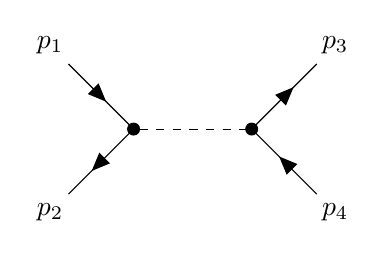
\begin{tikzpicture}[baseline=(c1.base)]
			\begin{feynman}
				\vertex [dot] (c1) at (0,0) {};
				\vertex [above left=of c1] (v1) {$p_1$};
				\vertex [below left=of c1] (v2) {$p_2$};
				\vertex [dot, right=of c1] (c2) {};
				\vertex [above right=of c2] (v3) {$p_3$};
				\vertex [below right=of c2] (v4) {$p_4$};
				%
				\diagram* {
					(v1) -- [fermion] (c1) -- [fermion] (v2);
                    (v4) -- [fermion] (c2) -- [fermion] (v3);
					(c1) -- [scalar] (c2);
				};
			\end{feynman} 
		\end{tikzpicture} ~ - ~ 
		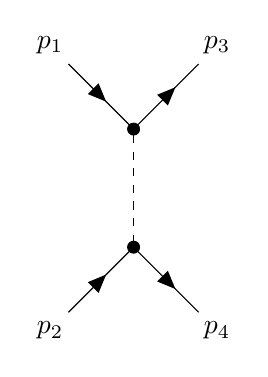
\begin{tikzpicture}[vertical'=c1 to c2, baseline=($0.5*(c1)+0.5*(c2)$)]
			\begin{feynman}
				\vertex [dot] (c1) {};
				\vertex [dot, below=of c1] (c2) {};
				\vertex [above left=of c1] (v1) {$p_1$};
				\vertex [above right=of c1] (v4) {$p_3$};
				\vertex [below left=of c2] (v2) {$p_2$};
				\vertex [below right=of c2] (v3) {$p_4$};
				%
				\diagram* {
					(v1) -- [fermion] (c1) -- [fermion] (v4) ;
					(c1) -- [scalar] (c2);
					(v2) -- [fermion] (c2) -- [fermion] (v3) ;
				};
			\end{feynman} 
		\end{tikzpicture} ~ = ~ i\mathcal{M}_s - i\mathcal{M}_u \, .
	\end{align}
    Observe that the two diagrams have a difference of a minus sign
    since in Eq.~\eqref{u_contraction} we moved $\sbar{\psi}(x)$ of two spaces to the right, while $\psi(x)$ must be moved of one space to the right, so we are left with a minus sign.  The reason why also $\psi(x)$ must be moved is that all the external state contractions must be done in the same order\footnote{this is related to the fact that we can define $|f(p_1), \sbar{f}(p_2)\rangle \sim \acon_{\vp_1,s} \bcon_{\vp_2,s}\ket{0}$ or $|f(p_1), \sbar{f}(p_2)\rangle \sim \bcon_{\vp_1,s} \acon_{\vp_2,s} \ket{0}$. Both definitions are possible but differ by a minus sign.}: in Eq.~\eqref{s_contraction} we applied to the final particles first $\sbar{\psi}$ and then $\psi$.
    However, in Eq.~\eqref{u_contraction} the fields are placed in the opposite order.
    Therefore, in order to be consistent with the choice done in Eq.~\eqref{s_contraction}, we have to exchange $\psi(x)$ and $\sbar{\psi}(y)$, getting an extra minus sign.
    %
    Other than these two contractions, we can have the cases in which $x$ and $y$ are exchanged.
        Since they give contributions identical to Eqs.~\eqref{s_contraction} and \eqref{u_contraction} (we have to exchange an even number of fermion fields), we can just cancel the prefactor $1/2!$ in Eq.~\eqref{wick_contracion} and forget about such diagrams.
        Considering just the contraction in Eq.~\eqref{s_contraction} (for the other one the derivation is identical), we find
        \begin{align}
            &\bra{f(p_3),\sbar{f}(p_4)}iT \ket{f(p_1), \sbar{f}(p_2)} \notag \\
            = &\; (ig)^2 \int \rmd^4x \; \rmd^4y \; D(x-y) \,e^{i(p_3+p_4) x} \, \sbar{u}^{s_3}(\vp_3) v^{s_4}(\vp_4)  \sbar{v}^{s_2}(\vp_2) u^{s_1}(\vp_1)e^{-i(p_1+p_2) y}\label{ciao}\,.
        \end{align}
        Inserting Eq.~\eqref{scalar_propagator} into Eq.~\eqref{ciao} we obtain
        \begin{align}
            &\bra{f(p_3),\sbar{f}(p_4)}iT \ket{f(p_1), \sbar{f}(p_2)} \notag \\
            = &\; (ig)^2 \int \frac{\rmd^4 q}{(2\pi)^4} \rmd^4x \; \rmd^4y \; \frac{i}{q^2 - M^2 + i\epsilon} \, e^{i(p_3+p_4 - q) x} \, \sbar{u}^{s_3}(\vp_3) v^{s_4}(\vp_4)  \sbar{v}^{s_2}(\vp_2) u^{s_1}(\vp_1)e^{-i(p_1+p_2-q) y}\notag \\
            = &\; (ig)^2 \int \frac{\rmd^4 q}{(2\pi)^4} \frac{i}{q^2 - M^2 + i\epsilon} \sbar{u}^{s_3}(\vp_3) v^{s_4}(\vp_4)  \sbar{v}^{s_2}(\vp_2) u^{s_1}(\vp_1) \notag \\ 
            & \times (2\pi)^4\delta^{(4)}(q - p_1 - p_2) (2\pi)^4\delta^{(4)}(q - p_3 - p_4) \notag \\
            = &\; i\mathcal{M}\left( p_1, p_2, p_3, p_4\right) (2 \pi)^4 \delta^{(4)}(p_1 + p_2 - p_3 - p_4)\,,
        \end{align}
        with
        \begin{equation}
            i \mathcal{M} \left( p_1, p_2, p_3, p_4\right) = (ig)^2 \frac{i}{q^2 - M^2 + i\epsilon} \sbar{u}^{s_3}(\vp_3) v^{s_4}(\vp_4)  \sbar{v}^{s_2}(\vp_2) u^{s_1}(\vp_1) \, .
        \end{equation}
        In conclusion, we have found that the Feynman rules of the theory are
	\begin{itemize}
		\item \textbf{External lines}
    \begin{align}
	 &
	\begin{tikzpicture}[baseline=(v1.base)]
		\begin{feynman}
			\vertex (v1) at (0,0);
			\vertex [dot, right=of v1] (v2) {};
			%
			\diagram {
				(v1) -- [scalar, momentum=$p$] (v2);
			};
		\end{feynman} 
	\end{tikzpicture} ~ = 1 \,, 
	&
	 &
	\begin{tikzpicture}[baseline=(v1.base)]
		\begin{feynman}
			\vertex [dot] (v1) at (0,0) {};
			\vertex [right=of v1] (v2);
			%
			\diagram {
				(v1) -- [scalar, momentum=$p$] (v2);
			};
		\end{feynman} 
	\end{tikzpicture} ~ = 1 \,, \\
	% ---------------------------------------------
	 &
	\begin{tikzpicture}[baseline=(v1.base)]
		\begin{feynman}
			\vertex (v1) at (0,0);
			\vertex [dot, right=of v1] (v2) {};
			%
			\diagram {
				(v1) -- [fermion, edge label=$p$] (v2);
			};
		\end{feynman} 
	\end{tikzpicture} ~ = u^s(\vp) \,, 
	&
	 &
	\begin{tikzpicture}[baseline=(v1.base)]
		\begin{feynman}
			\vertex [dot] (v1) at (0,0) {};
			\vertex [right=of v1] (v2);
			%
			\diagram {
				(v1) -- [fermion, edge label=$p$] (v2);
			};
		\end{feynman} 
	\end{tikzpicture} ~ = \bar{u}^s(\vp) \,, \\
	% ---------------------------------------------
	 &
	\begin{tikzpicture}[baseline=(v1.base)]
		\begin{feynman}
			\vertex (v1) at (0,0);
			\vertex [dot, right=of v1] (v2) {};
			%
			\diagram {
				(v2) -- [fermion, edge label'=$p$] (v1);
			};
		\end{feynman} 
	\end{tikzpicture} ~ = \bar{v}^s(\vp) \,, 
	&
	 &
	\begin{tikzpicture}[baseline=(v1.base)]
		\begin{feynman}
			\vertex [dot] (v1) at (0,0) {};
			\vertex [right=of v1] (v2);
			%
			\diagram {
				(v2) -- [fermion, edge label'=$p$] (v1);
			};
		\end{feynman} 
	\end{tikzpicture} ~ = v^s(\vp) \,,
    \end{align}

    \item \textbf{Propagators}
	\begin{align}
    &
	\begin{tikzpicture}[baseline=(c.base)]
		\begin{feynman}
			\vertex [dot] (c) at (0,0) {};
			\vertex [dot] [right=of c] (r) {} ;
			%
			\diagram {
				(c) --[scalar, edge label=$q$] (r);
			};
		\end{feynman} 
	\end{tikzpicture} ~ = ~ \frac{i}{q^2-M^2+i\epsilon} \,,
    %
	&& \text{scalar propagator}\,, \\
    % ---------------------------------------------
	&
	\begin{tikzpicture}[baseline=(c.base)]
		\begin{feynman}
			\vertex [dot] (c) at (0,0) {};
			\vertex [dot] [right=of c] (r) {} ;
			%
			\diagram {
				(c) --[fermion, edge label=$q$] (r);
			};
		\end{feynman} 
	\end{tikzpicture} ~ = ~ \frac{i(\slashed{q}+m)}{q^2-m^2+i\epsilon} \,,
    %
    && \text{fermion propagator}\,,
    \end{align}

    \item \textbf{Vertex}
	\begin{equation}
		\begin{tikzpicture}[baseline=(c.base)]
			\begin{feynman}
				\vertex [dot] (c) at (0,0) {};
				\vertex [above left=of c] (v1);
				\vertex [below left=of c] (v2);
				\vertex [right=of c] (v3);
				%
				\diagram {
					(v1) --[fermion] (c);
					(c) -- [fermion] (v2);
					(c) -- [scalar] (v3);
				};
			\end{feynman} 
		\end{tikzpicture} ~ = ~ i g \, .
	\end{equation}
    \end{itemize}

        \item In this case, using that the covariant derivative is defined as
        \begin{equation}
            D_\mu = \partial_\mu + ie A_\mu \,,
        \end{equation}
        we can rewrite $\La_2$ as
        \begin{equation}
        \label{L_2_new}
            \La_2 = -\frac{1}{4} F_{\mu \nu} F^{\mu \nu} + \partial^\mu \phi^* \partial_\mu \phi - m^2 \phi^* \phi + ie \left(   A^\mu \partial_\mu \phi^* \phi - A_\mu \phi^* \partial^\mu \phi \right) +e^2 A^\mu A_\mu \phi^* \phi \,.
        \end{equation}
        The first three terms of Eq.~\eqref{L_2_new} correspond to the kinetic terms of the photon and of the complex scalars.
        Following the derivation of the previous point one finds
        \begin{itemize}
		\item \textbf{External lines}
    \begin{align}
	\begin{tikzpicture}[baseline=(v1.base)]
		\begin{feynman}
			\vertex (v1) at (0,0);
			\vertex [dot, right=of v1] (v2) {};
			%
			\diagram {
				(v1) -- [charged scalar, edge label=$p$] (v2);
			};
		\end{feynman} 
	\end{tikzpicture} ~ = & ~ 1 \,, 
	&
	 &
	\begin{tikzpicture}[baseline=(v1.base)]
		\begin{feynman}
			\vertex [dot] (v1) at (0,0) {};
			\vertex [right=of v1] (v2);
			%
			\diagram {
				(v1) -- [charged scalar, edge label=$p$] (v2);
			};
		\end{feynman} 
	\end{tikzpicture} ~ = 1 \,, \\
	% ---------------------------------------------
	\begin{tikzpicture}[baseline=(v1.base)]
		\begin{feynman}
			\vertex (v1) at (0,0) {\(\mu\)};
			\vertex [dot, right=of v1] (v2) {};
			%
			\diagram {
				(v1) -- [boson, edge label=$p$] (v2);
			};
		\end{feynman} 
	\end{tikzpicture} ~ = & ~ \epsilon_\mu(\vp, \lambda) \,, 
	&&
	\begin{tikzpicture}[baseline=(v1.base)]
		\begin{feynman}
			\vertex [dot] (v1) at (0,0) {};
			\vertex [right=of v1] (v2) {\(\mu\)};
			%
			\diagram {
				(v1) -- [boson, edge label=$p$] (v2);
			};
		\end{feynman} 
	\end{tikzpicture} = \epsilon_\mu^*(\vp, \lambda) \,,
	% ---------------------------------------------
    \end{align}

    \item \textbf{Propagators}
	\begin{align}
	\begin{tikzpicture}[baseline=(c.base)]
		\begin{feynman}
			\vertex [dot] (c) at (0,0) {};
			\vertex [dot] [right=of c] (r) {} ;
			%
			\diagram {
				(c) --[charged scalar, edge label=$q$] (r);
			};
		\end{feynman} 
	\end{tikzpicture} ~ = & ~ \frac{i}{q^2-M^2+i\epsilon} \,, 
	%
    && \text{scalar propagator}\,, \\
    % ---------------------------------------------
	\begin{tikzpicture}[baseline=(c.base)]
		\begin{feynman}
			\vertex [dot, label=90:$\mu$] (c) at (0,0) {};
			\vertex [dot, label=90:$\nu$] [right=of c] (r) {} ;
			%
			\diagram {
				(c) --[boson, edge label=$q$] (r);
			};
		\end{feynman} 
	\end{tikzpicture} ~ = & ~ -\frac{i}{q^2+i\epsilon}\left(g_{\mu \nu} - (1 - \xi) \frac{q_\mu q_\nu}{q^2}\right) \,,
    %
    && \text{photon propagator} \,.
    \end{align}

\item  \textbf{Vertices} 

        Regarding the vertices, the interaction Lagrangian is
        \begin{equation}
        \label{L_2_int}
            \La_{2,int} = ie \left(   A^\mu \partial_\mu \phi^* \phi - A_\mu \phi^* \partial^\mu \phi \right) +e^2 A^\mu A_\mu \phi^* \phi\,.
        \end{equation}
        The second term gives an interaction between two photons and two scalars.
        It is easy to get that the last term of Eq.~\eqref{L_2_int} corresponds to the vertex
        \begin{equation}
		\begin{tikzpicture}[baseline=(c.base)]
			\begin{feynman}
				\vertex [dot] (c) at (0,0) {};
				\vertex [above left=of c] (v1) {\(\mu\)};
				\vertex [below left=of c] (v2) {\(\nu\)};
				\vertex [above right=of c] (v3);
                \vertex [below right=of c] (v4) ;
				%
				\diagram {
					(v1) --[boson] (c);
					(c) -- [boson] (v2);
					(c) -- [charged scalar] (v3);
                    (v4) -- [charged scalar] (c);
				};
			\end{feynman} 
		\end{tikzpicture} ~ = ~ 2 i e^2 \g^{\mu \nu} \,.
	\end{equation}
    The factor of 2 comes from the exchanging of the photon field. The first term of Eq.~\eqref{L_2_int} gives an interaction between two scalars and a photon. It reads
 \begin{equation}
		\begin{tikzpicture}[baseline=(c.base)]
			\begin{feynman}
				\vertex [dot] (c) at (0,0) {};
				\vertex [above left=of c] (v1);
				\vertex [below left=of c] (v2);
				\vertex [right=of c] (v3) {\(\mu\)} ;
				%
				\diagram {
					(v1) --[charged scalar] (c);
					(c) -- [charged scalar] (v2);
					(c) -- [boson] (v3);
				};
			\end{feynman} 
		\end{tikzpicture} = ~ i e (p_1^\mu - p_2^\mu) \,.
	\end{equation}
    The momenta come from applying the derivative to the initial state scalars. Since we have that
    \begin{align}
        &\wick{  \c \phi(x) \ket{\c s(p)} } = e^{-ipx} \ket{0} \, , \\
        &\wick{  \c \phi^*(x) \ket{\sbar{\c s}(p)} } = e^{-ipx} \ket{0} \, , \\
        &\wick{  \langle \c s(p)| \c \phi^*(x) } = e^{ipx} \bra{0} \, , \\
        &\wick{  \langle \sbar{\c s}(p)| \c \phi^*(x) } = e^{ipx} \bra{0} \, , 
    \end{align}
    each derivative yields a factor of $-ip^\mu$. In the case where the scalar is in the outgoing state, the factor becomes $ip^\mu$ and so we have to invert the sign of the momentum.
    \end{itemize}
    
    \item In this case we have massless fermions coupled by an interaction Lagrangian of the form
    \begin{equation}
    \label{lint_3}
    \begin{split}
        \La_I &=  G \sbar{\psi}_1 \gamma^\mu \psi_2 \sbar{\psi}_2 \gamma_\mu \psi_1 \\
              &= G \sbar{\psi}_{1,c} \left(\gamma^\mu\right)_{cd} \psi_{2,d} \sbar{\psi}_{2,b} \left(\gamma_\mu\right)_{ba} \psi_{1,a}\,,
    \end{split}
    \end{equation}
    where in the last line we spelled out explicitly the Dirac indices.
    The external lines and the propagators are the same as in point a), and are given by

    \begin{itemize}
		\item \textbf{External lines}
    \begin{align}
	% ---------------------------------------------
	 &
	\begin{tikzpicture}[baseline=(v1.base)]
		\begin{feynman}
			\vertex (v1) at (0,0);
			\vertex [dot, right=of v1] (v2) {};
			%
			\diagram {
				(v1) -- [fermion, edge label=$p$] (v2);
			};
		\end{feynman} 
	\end{tikzpicture} ~ = u_1^s(\vp) \,, 
	&
	 &
	\begin{tikzpicture}[baseline=(v1.base)]
		\begin{feynman}
			\vertex [dot] (v1) at (0,0) {};
			\vertex [right=of v1] (v2);
			%
			\diagram {
				(v1) -- [fermion, edge label=$p$] (v2);
			};
		\end{feynman} 
	\end{tikzpicture} ~ = \bar{u}_1^s(\vp) \,, \\
	% ---------------------------------------------
	 &
	\begin{tikzpicture}[baseline=(v1.base)]
		\begin{feynman}
			\vertex (v1) at (0,0);
			\vertex [dot, right=of v1] (v2) {};
			%
			\diagram {
				(v2) -- [fermion, edge label'=$p$] (v1);
			};
		\end{feynman} 
	\end{tikzpicture} ~ = \bar{v}_1^s(\vp) \,, 
	&
	 &
	\begin{tikzpicture}[baseline=(v1.base)]
		\begin{feynman}
			\vertex [dot] (v1) at (0,0) {};
			\vertex [right=of v1] (v2);
			%
			\diagram {
				(v2) -- [fermion, edge label'=$p$] (v1);
			};
		\end{feynman} 
	\end{tikzpicture} ~ = v_1^s(\vp) \,, \\
 % ---------------------------------------------
	 &
	\begin{tikzpicture}[baseline=(v1.base)]
		\begin{feynman}
			\vertex (v1) at (0,0);
			\vertex [dot, right=of v1] (v2) {};
			%
			\diagram {
				(v1) -- [red, fermion, edge label=$p$] (v2);
			};
		\end{feynman} 
	\end{tikzpicture} ~ = u_2^s(\vp) \,, 
	&
	 &
	\begin{tikzpicture}[baseline=(v1.base)]
		\begin{feynman}
			\vertex [dot] (v1) at (0,0) {};
			\vertex [right=of v1] (v2);
			%
			\diagram {
				(v1) -- [red, fermion, edge label=$p$] (v2);
			};
		\end{feynman} 
	\end{tikzpicture} ~ = \bar{u}_2^s(\vp) \,, \\
	% ---------------------------------------------
	 &
	\begin{tikzpicture}[baseline=(v1.base)]
		\begin{feynman}
			\vertex (v1) at (0,0);
			\vertex [dot, right=of v1] (v2) {};
			%
			\diagram {
				(v2) -- [red, fermion, edge label'=$p$] (v1);
			};
		\end{feynman} 
	\end{tikzpicture} ~ = \bar{v}_2^s(\vp) \,, 
	&
	 &
	\begin{tikzpicture}[baseline=(v1.base)]
		\begin{feynman}
			\vertex [dot] (v1) at (0,0) {};
			\vertex [right=of v1] (v2);
			%
			\diagram {
				(v2) -- [red, fermion, edge label'=$p$] (v1);
			};
		\end{feynman} 
	\end{tikzpicture} ~ = v_2^s(\vp) \,,
    \end{align}

    \item \textbf{Propagators}
	\begin{align}
	&
	\begin{tikzpicture}[baseline=(c.base)]
		\begin{feynman}
			\vertex [dot] (c) at (0,0) {};
			\vertex [dot] [right=of c] (r) {} ;
			%
			\diagram {
				(c) --[fermion, edge label=$q$] (r);
			};
		\end{feynman} 
	\end{tikzpicture} ~ = ~ \frac{i\slashed{q}}{q^2+i\epsilon} \,,
    %
    && \text{$\psi_1$ propagator}\,, \\
        % ---------------------------------------------
	&
	\begin{tikzpicture}[baseline=(c.base)]
		\begin{feynman}
			\vertex [dot] (c) at (0,0) {};
			\vertex [dot] [right=of c] (r) {} ;
			%
			\diagram {
				(c) --[red, fermion, edge label=$q$] (r);
			};
		\end{feynman} 
	\end{tikzpicture} ~ = ~ \frac{i\slashed{q}}{q^2+i\epsilon} \,,
    %
    && \text{$\psi_2$ propagator} \,,
    \end{align}
    where black lines and red lines denote fermions of type 1 and type 2 respectively. 
    \item  \textbf{Vertices} 
    
    Regarding the vertices, we can observe that the interaction Lagrangian in Eq.\eqref{lint_3} is a 4-fermion interaction,
    with two fermions of each type.
    The two possible vertices are
        \begin{equation}
		\begin{tikzpicture}[baseline=(c.base)]
			\begin{feynman}
				\vertex [dot] (c) at (0,0) {};
				\vertex [above left=of c] (v1) {\(a\)};
				\vertex [below left=of c] (v2) {\(b\)};
				\vertex [above right=of c] (v3) {\(c\)};
                \vertex [below right=of c] (v4) {\(d\)};
				%
				\diagram {
					(v1) --[fermion] (c);
					(c) -- [red, fermion] (v2);
					(c) -- [fermion] (v3);
                    (v4) -- [red, fermion] (c);
				};
			\end{feynman} 
		\end{tikzpicture} ~ = ~ i G \left(\gamma^\mu\right)_{cd} \left(\gamma_\mu\right)_{ba} 
	\end{equation}
    and
        \begin{equation}
		\begin{tikzpicture}[baseline=(c.base)]
			\begin{feynman}
				\vertex [dot] (c) at (0,0) {};
				\vertex [above left=of c] (v1) {\(a\)};
				\vertex [below left=of c] (v2) {\(b\)};
				\vertex [above right=of c] (v3) {\(c\)};
                \vertex [below right=of c] (v4) {\(d\)};
				%
				\diagram {
					(v1) --[fermion] (c);
					(v2) -- [red, fermion] (c);
					(c) -- [fermion] (v3);
                    (c) -- [red, fermion] (v4);
				};
			\end{feynman} 
		\end{tikzpicture} ~ = ~ i G \left(\gamma^\mu\right)_{cb} \left(\gamma_\mu\right)_{da} \,.
	\end{equation}
    \end{itemize}
    \item Left to the reader.
    \end{enumerate}
    $ $
\end{sol}




\end{document}
